\documentclass[11pt, oneside]{article}   	% use "amsart" instead of "article" for AMSLaTeX format
\usepackage{geometry}                		% See geometry.pdf to learn the layout options. There are lots.
\geometry{letterpaper}                   		% ... or a4paper or a5paper or ... 
%\geometry{landscape}                		% Activate for rotated page geometry
\usepackage[parfill]{parskip}    		% Activate to begin paragraphs with an empty line rather than an indent
\usepackage{graphicx}				% Use pdf, png, jpg, or eps§ with pdflatex; use eps in DVI mode
								% TeX will automatically convert eps --> pdf in pdflatex		
\usepackage[margin=10pt,font=footnotesize,labelfont=bf]{caption}
\usepackage{subcaption}
\usepackage{float}
\usepackage{amssymb}
\usepackage{amsmath}
\usepackage{bm}
\usepackage{bbm}
\usepackage{mleftright}
\usepackage{todonotes}

%\bibliographystyle{apalike}

\graphicspath{ {images/} }


\newcommand{\sotodo}{\todo[color=green]}
\newcommand{\sotodoinline}{\todo[color=green,inline=true]}
\newcommand{\bstodo}{\todo[color=pink]}
\newcommand{\bstodoinline}{\todo[color=pink,inline=true]}


%SetFonts

%SetFonts

\usepackage[square,numbers]{natbib}
\usepackage{url}
%\bibliographystyle{elsarticle-harv}
\bibliographystyle{plain}

\newcommand{\bigO}{\mathcal{O}}
\newcommand{\half}{\frac{1}{2}}
\newcommand{\R}{\mathbb{R}}
\newcommand{\C}{\mathbb{C}}
\newcommand{\Z}{\mathbb{Z}}
\newcommand{\N}{\mathbb{N}}
\newcommand{\No}{\mathbb{N}_0}
\newcommand{\Ylm}{Y^m_l}
\newcommand{\Ylmfull}{Y^m_l(\theta,\varphi)}
\newcommand{\Plm}{\jac^m_l}
\newcommand{\costheta}{\cos\theta}
\newcommand{\sintheta}{\sin\theta}
\newcommand{\cosphi}{\cos\varphi}
\newcommand{\sinphi}{\sin\varphi}
\newcommand{\eimphi}{e^{im\varphi}}
\newcommand{\alphalm}{\alpha^m_l}
\newcommand{\clm}{c^m_l}
\newcommand{\ctilde}{\tilde{c}^m_l}
\newcommand{\ctildemod}{\tilde{c}^{|m|}_l}
\newcommand{\chat}{\hat{c}^m_l}
\newcommand{\chatmod}{\hat{c}^{|m|}_l}
\newcommand{\ddx}{\frac{\mathrm{d}}{\mathrm{d}x}}
\newcommand{\ddy}{\frac{\mathrm{d}}{\mathrm{d}y}}
\newcommand{\pddx}{\frac{\partial}{\partial x}}
\newcommand{\pddy}{\frac{\partial}{\partial y}}
\newcommand{\pddn}{\frac{\partial}{\partial n}}
\newcommand{\dmdxm}{\frac{\mathrm{d}^m}{\mathrm{d}x^m}}

\newcommand{\Atilde}{\tilde{A}_{l,m}}
\newcommand{\Btilde}{\tilde{B}_{l,m}}
\newcommand{\Dtilde}{\tilde{D}_{l,m}}
\newcommand{\Etilde}{\tilde{E}_{l,m}}
\newcommand{\Ftilde}{\tilde{F}_{l,m}}
\newcommand{\Gtilde}{\tilde{G}_{l,m}}
\newcommand{\Alm}{A_{l,m}}
\newcommand{\Blm}{B_{l,m}}
\newcommand{\Dlm}{D_{l,m}}
\newcommand{\Elm}{E_{l,m}}
\newcommand{\Flm}{F_{l,m}}
\newcommand{\Glm}{G_{l,m}}

\newcommand{\xione}{\xi^{(1)}_{n, \lambda}}
\newcommand{\xitwo}{\xi^{(2)}_{n, \lambda}}
\newcommand{\xithree}{\xi^{(3)}_{n, \lambda}}
\newcommand{\xifour}{\xi^{(4)}_{n, \lambda}}

\newcommand{\bigP}{\mathbb{P}}
\newcommand{\Pl}{\mathbb{P}_l}
\newcommand{\gradP}{T\mathbb{P}}
\newcommand{\gradPl}{T\mathbb{P}_l}
\newcommand{\gradY}{\nabla Y}
\newcommand{\gradYlm}{\nabla Y^m_l}
\newcommand{\gradpY}{\nabla^\perp Y}
\newcommand{\gradpYlm}{\nabla^\perp Y^m_l}

\newcommand{\Dlt}{D^\top_l}

\newcommand{\curlyy}{\bm{\mathcal{Y}}}
\newcommand{\blone}{\beta_{l, 1}}
\newcommand{\blzero}{\beta_{l, 0}}
\newcommand{\blmone}{\beta_{l, -1}}
\newcommand{\chivec}{\bm{\chi}_{1,m_s}}
\newcommand{\cgcoeff}{\mathcal{C}}

\newcommand{\alm}{a_{l,m}}
\newcommand{\blm}{b_{l,m}}
\newcommand{\dlm}{d_{l,m}}
\newcommand{\elm}{e_{l,m}}
\newcommand{\flm}{f_{l,m}}
\newcommand{\glm}{g_{l,m}}
\newcommand{\hlm}{h_{l,m}}
\newcommand{\jlm}{j_{l,m}}
\newcommand{\klm}{k_{l,m}}
\newcommand{\almperp}{a_{l,m}^\perp}
\newcommand{\blmperp}{b_{l,m}^\perp}
\newcommand{\dlmperp}{d_{l,m}^\perp}
\newcommand{\elmperp}{e_{l,m}^\perp}
\newcommand{\flmperp}{f_{l,m}^\perp}
\newcommand{\glmperp}{g_{l,m}^\perp}
\newcommand{\hlmperp}{h_{l,m}^\perp}
\newcommand{\jlmperp}{j_{l,m}^\perp}
\newcommand{\klmperp}{k_{l,m}^\perp}

\newcommand{\unitvec}{\hat{\bm{k}}}

\newcommand{\hdop}{H}
\newcommand{\bighdop}{\mathbb{\hdop}}
\newcommand{\hdopnk}{\hdop_{n,k}}
\newcommand{\hdopnkab}{\hdop_{n,k}^{(a,b)}}
\newcommand{\hdopab}{\hdop^{(a,b)}}
\newcommand{\Wab}{{W^{(a,b)}}}
\newcommand{\hdopmj}{\hdop_{m,j}}
\newcommand{\hdopmjab}{\hdop_{m,j}^{(a,b)}}
\newcommand{\alphaab}{\alpha^{(a,b)}}
\newcommand{\betaab}{\beta^{(a,b)}}
\newcommand{\bighdopab}{\bighdop^{(a,b)}}
\newcommand{\Dnt}{D^\top_n}
\newcommand{\Wii}{W^{(1,1)}}
\newcommand{\hdopii}{\hdop^{(1,1)}}
\newcommand{\bighdopii}{{\mathbb{\hdop}^{(1,1)}}}
\newcommand{\hdopoo}{\hdop^{(0,0)}}
\newcommand{\bighdopoo}{{\mathbb{\hdop}^{(0,0)}}}
\newcommand{\hdopoi}{\hdop^{(0,1)}}
\newcommand{\hdopio}{\hdop^{(1,0)}}
%\newcommand{\jac}{{\tilde P}}
\newcommand{\jac}{{P}}
\newcommand{\genjac}{R}
\newcommand{\genjacnmk}{\genjac_{n-k}}
\newcommand{\genjacmmj}{\genjac_{m-j}}
\newcommand{\genjacw}{w_\genjac}
\newcommand{\jacw}{w_P}
\newcommand{\normgenjac}{\omega_\genjac}
\newcommand{\normjac}{\omega_P}

\newcommand{\dx}{\frac{\partial}{\partial x}}
\newcommand{\dy}{\frac{\partial}{\partial y}}
\newcommand{\laplacewii}{\Delta_W^{(1,1)\to(1,1)}}
\newcommand{\laplacewtt}{\Delta_W^{(2,2)\to(0,0)}}
\newcommand{\laplaceoo}{\Delta^{(0,0)\to(2,2)}}
\newcommand{\biharmonic}{_2\Delta_W^{(2,2)\to(2,2)}}

\newcommand{\element}{\tau}
\newcommand{\refelement}{\hat{\tau}}
\newcommand{\FEset}{\mathcal{T}}
\newcommand{\bigW}{\mathbb{W}}
\newcommand{\bigWab}{\mathbb{W}^{(a,b)}}
\newcommand{\bigWii}{{\mathbb{W}^{(1,1)}}}
\newcommand{\bigQ}{\mathbb{Q}}
\newcommand{\bigQab}{\bigQ^{(a,b)}}


\newcommand{\hdopnkabc}{\hdop_{n,k}^{(a,b,c)}}
\newcommand{\hdopabc}{\hdop^{(a,b,c)}}
\newcommand{\Wabc}{{W^{(a,b,c)}}}
\newcommand{\hdopmjabc}{\hdop_{m,j}^{(a,b,c)}}
\newcommand{\alphaabc}{\alpha^{(a,b,c)}}
\newcommand{\betaabc}{\beta^{(a,b,c)}}
\newcommand{\bighdopabc}{\bighdop^{(a,b,c)}}
\newcommand{\Wiii}{W^{(1,1,1)}}
\newcommand{\hdopiii}{\hdop^{(1,1,1)}}
\newcommand{\bighdopiii}{{\mathbb{\hdop}^{(1,1,1)}}}
\newcommand{\hdopooo}{\hdop^{(0,0,0)}}
\newcommand{\bighdopooo}{{\mathbb{\hdop}^{(0,0,0)}}}
\newcommand{\hdopooi}{\hdop^{(0,0,1)}}
\newcommand{\hdopiio}{\hdop^{(1,1,0)}}
\newcommand{\laplacewiii}{\Delta_W^{(1,1,1)\to(1,1,1)}}
\newcommand{\laplacewttt}{\Delta_W^{(2,2,2)\to(0,0,0)}}
\newcommand{\laplaceooo}{\Delta^{(0,0,0)\to(2,2,2)}}
\newcommand{\biharmonictwo}{_2\Delta_W^{(2,2,2)\to(2,2,2)}}
\newcommand{\bigWiii}{{\mathbb{W}^{(1,1,1)}}}
\newcommand{\bigWabc}{\mathbb{W}^{(a,b,c)}}

\newcommand{\alphaabcd}{\alpha^{(a,b,c,d)}}
\newcommand{\betaabcd}{\beta^{(a,b,c,d)}}
\newcommand{\hdopnkabcd}{\hdop_{n,k}^{(a,b,c,d)}}
\newcommand{\hdopabcd}{\hdop^{(a,b,c,d)}}
\newcommand{\Wabcd}{{W^{(a,b,c,d)}}}
\newcommand{\hdopmjabcd}{\hdop_{m,j}^{(a,b,c,d)}}
\newcommand{\bighdopabcd}{\bighdop^{(a,b,c,d)}}
\newcommand{\bigWabcd}{\mathbb{W}^{(a,b,c,d)}}

\newcommand{\genjact}{\tilde{\genjac}}
\newcommand{\genjactnmk}{\genjact_{n-k}}
\newcommand{\genjactmmj}{\genjact_{m-j}}
\newcommand{\genjactw}{w_{\genjact}}
\newcommand{\normgenjact}{\omega_{\genjact}}

% Spherical Cap commands
\newcommand{\scop}{Q}
\newcommand{\scopnki}{\scop_{n,k,i}}
\newcommand{\scopmjh}{\scop_{m,j,h}}
\newcommand{\scopa}{\scop^{(a)}}
\newcommand{\scopnkia}{\scopnki^{(a)}}
\newcommand{\scopmjha}{\scopmjh^{(a)}}
\newcommand{\bigscop}{{\mathbb{Q}}}
\newcommand{\bigscopa}{\bigscop^{(a)}}
\newcommand{\bigscopN}{\bigscop_{N}}
\newcommand{\bigscopNa}{\bigscopa_{N}}
\newcommand{\bigscopNka}{\bigscopa_{N,k}}
\newcommand{\bigscopt}{\mathbb{\tilde{Q}}}
\newcommand{\bigscopta}{\bigscopt^{(a)}}
\newcommand{\bigscoptn}{\bigscopt_{n}}
\newcommand{\bigscoptna}{\bigscopta_{n}}
\newcommand{\xvec}{\mathbf{x}}
\newcommand{\ch}{Y}
\newcommand{\chki}{\ch_{k,i}}
\newcommand{\chjh}{\ch_{j,h}}
\newcommand{\chkitheta}{\ch_{k,i}(\theta)}
\newcommand{\alphaa}{\alpha^{(a)}}
\newcommand{\betaa}{\beta^{(a)}}
\newcommand{\gammaa}{\gamma^{(a)}}
\newcommand{\Wa}{W^{(a)}}
\newcommand{\bigWNa}{\mathbb{W}_N^{(a)}}
\newcommand{\ppphi}{\frac{\partial}{\partial \phi}}
\newcommand{\ppz}{\frac{\partial}{\partial z}}
\newcommand{\rhoppphi}{\rho \ppphi}
\newcommand{\pptheta}{\frac{\partial}{\partial \theta}}
\newcommand{\bigWNi}{\mathbb{W}_N^{(1)}}
\newcommand{\scopi}{\scop^{(1)}}
\newcommand{\scopnkii}{\scopnki^{(1)}}
\newcommand{\bigWNo}{\mathbb{W}_N^{(0)}}
\newcommand{\scopo}{\scop^{(0)}}
\newcommand{\scopnkio}{\scopnki^{(0)}}
\newcommand{\bigscopi}{\bigscop^{(1)}}
\newcommand{\bigscopNi}{\bigscopi_{N}}
\newcommand{\bigscopNki}{\bigscopi_{N,k}}
\newcommand{\bigscopo}{\bigscop^{(0)}}
\newcommand{\bigscopNo}{\bigscopo_{N}}
\newcommand{\bigscopNko}{\bigscopo_{N,k}}

% Tangent space
\newcommand{\tangentspace}{{\Omega_T}}
\newcommand{\phivec}{\hat{\bm{\phi}}}
\newcommand{\thetavec}{\hat{\bm{\theta}}}
\newcommand{\bigtsop}{\mathbb{T}}
\newcommand{\bigtsopt}{\tilde{\bigtsop}}
\newcommand{\bigtsoptn}{\bigtsopt_n}
\newcommand{\bigtsopN}{\bigtsop_N}
\newcommand{\bigtsopNk}{\bigtsop_{N,k}}
\newcommand{\tsopi}{\bm{\Phi}}
\newcommand{\tsopii}{\bm{\Psi}}
\newcommand{\tsopiN}{\tsopi_N}
\newcommand{\tsopiiN}{\tsopii_N}
\newcommand{\tsopinki}{\tsopi_{n,k,i}}
\newcommand{\tsopiinki}{\tsopii_{n,k,i}}
\newcommand{\tsopinkit}{\tsopi_{n,k,i}^\top}
\newcommand{\tsopiinkit}{\tsopii_{n,k,i}\top}
\newcommand{\tsopit}{\tsopi^\top}
\newcommand{\tsopiit}{\tsopii^\top}
\newcommand{\rvec}{\hat{\bm{r}}}
\newcommand{\jacobimattangent}{{}^T\!J}
\newcommand{\jacobimattangentx}{\jacobimattangent_x}
\newcommand{\jacobimattangenty}{\jacobimattangent_y}
\newcommand{\jacobimattangentz}{\jacobimattangent_z}
\newcommand{\alphao}{\alpha^{(0)}}
\newcommand{\alphaonkj}{\alphao_{n,k,j}}
\newcommand{\betao}{\beta^{(0)}}
\newcommand{\betaonkj}{\betao_{n,k,j}}
\newcommand{\gammao}{\gamma^{(0)}}
\newcommand{\gammaonkj}{\gammao_{n,k,j}}





\usepackage{amsthm}

\newtheorem{proposition}{Proposition}
\newtheorem{lemma}{Lemma} 
\newtheorem{theorem}{Theorem} 
\newtheorem{definition}{Definition}
\newtheorem{condition}{Condition}
\newtheorem{algorithm}{Algorithm}
\newtheorem{corollary}{Corollary}

\def\condref#1{Condition~\ref{cond:#1}}


\def\addtab#1={#1\;&=}

\def\meeq#1{\def\ccr{\\\addtab}
%\tabskip=\@centering
 \begin{align*}
 \addtab#1
 \end{align*}
  }  
  
  \def\leqaddtab#1\leq{#1\;&\leq}
  \def\mleeq#1{\def\ccr{\\\addtab}
%\tabskip=\@centering
 \begin{align*}
 \leqaddtab#1
 \end{align*}
  }  


\def\vc#1{\mbox{\boldmath$#1$\unboldmath}}

\def\vcsmall#1{\mbox{\boldmath$\scriptstyle #1$\unboldmath}}

\def\vczero{{\mathbf 0}}


%\def\beginlist{\begin{itemize}}
%
%\def\endlist{\end{itemize}}


\def\pr(#1){\left({#1}\right)}
\def\br[#1]{\left[{#1}\right]}
\def\fbr[#1]{\!\left[{#1}\right]}
\def\set#1{\left\{{#1}\right\}}
\def\ip<#1>{\left\langle{#1}\right\rangle}
\def\iip<#1>{\left\langle\!\langle{#1}\right\rangle\!\rangle}

\def\norm#1{\left\| #1 \right\|}

\def\abs#1{\left|{#1}\right|}
\def\fpr(#1){\!\pr({#1})}

\def\Re{{\rm Re}\,}
\def\Im{{\rm Im}\,}

\def\floor#1{\left\lfloor#1\right\rfloor}
\def\ceil#1{\left\lceil#1\right\rceil}


\def\mapengine#1,#2.{\mapfunction{#1}\ifx\void#2\else\mapengine #2.\fi }

\def\map[#1]{\mapengine #1,\void.}

\def\mapenginesep_#1#2,#3.{\mapfunction{#2}\ifx\void#3\else#1\mapengine #3.\fi }

\def\mapsep_#1[#2]{\mapenginesep_{#1}#2,\void.}


\def\vcbr[#1]{\pr(#1)}


\def\bvect[#1,#2]{
{
\def\dots{\cdots}
\def\mapfunction##1{\ | \  ##1}
	\sopmatrix{
		 \,#1\map[#2]\,
	}
}
}

\def\vect[#1]{
{\def\dots{\ldots}
	\vcbr[{#1}]
}}

\def\vectt[#1]{
{\def\dots{\ldots}
	\vect[{#1}]^{\top}
}}

\def\Vectt[#1]{
{
\def\mapfunction##1{##1 \cr} 
\def\dots{\vdots}
	\begin{pmatrix}
		\map[#1]
	\end{pmatrix}
}}



\def\thetaB{\mbox{\boldmath$\theta$}}
\def\zetaB{\mbox{\boldmath$\zeta$}}


\def\newterm#1{{\it #1}\index{#1}}


\def\TT{{\mathbb T}}
\def\C{{\mathbb C}}
\def\R{{\mathbb R}}
\def\II{{\mathbb I}}
\def\F{{\mathcal F}}
\def\E{{\rm e}}
\def\I{{\rm i}}
\def\D{{\rm d}}
\def\dx{\D x}
\def\dy{\D y}
\def\CC{{\cal C}}
\def\DD{{\cal D}}
\def\U{{\mathbb U}}
\def\A{{\cal A}}
\def\K{{\cal K}}
\def\DTU{{\cal D}_{{\rm T} \rightarrow {\rm U}}}
\def\LL{{\cal L}}
\def\B{{\cal B}}
\def\T{{\cal T}}
\def\W{{\cal W}}


\def\tF_#1{{\tt F}_{#1}}
\def\Fm{\tF_m}
\def\Fab{\tF_{\alpha,\beta}}
\def\FC{\T}
\def\FCpmz{\FC^{\pm {\rm z}}}
\def\FCz{\FC^{\rm z}}

\def\tFC_#1{{\tt T}_{#1}}
\def\FCn{\tFC_n}

\def\rmz{{\rm z}}

\def\chapref#1{Chapter~\ref{Chapter:#1}}
\def\secref#1{Section~\ref{Section:#1}}
\def\exref#1{Exercise~\ref{Exercise:#1}}
\def\lmref#1{Lemma~\ref{Lemma:#1}}
\def\propref#1{Proposition~\ref{Proposition:#1}}
\def\warnref#1{Warning~\ref{Warning:#1}}
\def\thref#1{Theorem~\ref{Theorem:#1}}
\def\defref#1{Definition~\ref{Definition:#1}}
\def\probref#1{Problem~\ref{Problem:#1}}
\def\corref#1{Corollary~\ref{Corollary:#1}}
\def\appref#1{Appendix~\ref{Appendix:#1}}

\def\sgn{{\rm sgn}\,}
\def\Ai{{\rm Ai}\,}
\def\Bi{{\rm Bi}\,}
\def\wind{{\rm wind}\,}
\def\erf{{\rm erf}\,}
\def\erfc{{\rm erfc}\,}
\def\qqquad{\qquad\quad}
\def\qqqquad{\qquad\qquad}


\def\spand{\hbox{ and }}
\def\spodd{\hbox{ odd}}
\def\speven{\hbox{ even}}
\def\qand{\quad\hbox{and}\quad}
\def\qqand{\qquad\hbox{and}\qquad}
\def\qfor{\quad\hbox{for}\quad}
\def\qqfor{\qquad\hbox{for}\qquad}
\def\qas{\quad\hbox{as}\quad}
\def\qqas{\qquad\hbox{as}\qquad}
\def\qor{\quad\hbox{or}\quad}
\def\qqor{\qquad\hbox{or}\qquad}
\def\qqwhere{\qquad\hbox{where}\qquad}



%%% Words

\def\naive{na\"\i ve\xspace}
\def\Jmap{Joukowsky map\xspace}
\def\Mobius{M\"obius\xspace}
\def\Holder{H\"older\xspace}
\def\Mathematica{{\sc Mathematica}\xspace}
\def\apriori{apriori\xspace}
\def\WHf{Weiner--Hopf factorization\xspace}
\def\WHfs{Weiner--Hopf factorizations\xspace}

\def\Jup{J_\uparrow^{-1}}
\def\Jdown{J_\downarrow^{-1}}
\def\Jin{J_+^{-1}}
\def\Jout{J_-^{-1}}



\def\bD{\D\!\!\!^-}




\def\questionequals{= \!\!\!\!\!\!{\scriptstyle ? \atop }\,\,\,}

\def\elll#1{\ell^{\lambda,#1}}
\def\elllp{\ell^{\lambda,p}}
\def\elllRp{\ell^{(\lambda,R),p}}


\def\elllRpz_#1{\ell_{#1{\rm z}}^{(\lambda,R),p}}


\def\sopmatrix#1{\begin{pmatrix}#1\end{pmatrix}}

\def\socases#1{\begin{cases} #1 \end{cases}}


\def\Problem#1#2\par{\begin{problem}\label{pb:#1} #2\end{problem}}
\def\Theorem#1#2\par{\begin{theorem}\label{th:#1} #2\end{theorem}}
\def\Conjecture#1#2\par{\begin{conjecture}\label{conj:#1} #2\end{conjecture}}
\def\Proposition#1#2\par{\begin{proposition}\label{prop:#1} #2\end{proposition}}
\def\Definition#1#2\par{\begin{definition}\label{def:#1} #2\end{definition}}
\def\Corollary#1#2\par{\begin{corollary}\label{cr:#1} #2\end{corollary}}
\def\Lemma#1#2\par{\begin{lemma}\label{lm:#1} #2\end{lemma}}
\def\Example#1#2\par{\begin{example}\label{ex:#1} #2\end{example}}
\def\Remark #1\par{\begin{remark*}#1\end{remark*}}


\def\Proof{\begin{proof}}
\def\mqed{\end{proof}}


\def\Figuretwow[#1,#2]#3#4\par{
\begin{figure}[tb]
\begin{center}{
\includegraphics[width=#3]{Figures/#1}\includegraphics[width=#3]{Figures/#2}}
\end{center}
\caption{#4}\label{fig:#1} 
\end{figure}
}

%\usepackage{media9}
%\graphicspath{ {../sphere/plots} }



\title{Sparse spectral and $p$-finite element methods for partial differential equations on spherical caps}
\author{Ben Snowball, Sheehan Olver\thanks{Department of Mathematics, Imperial College, London, England}}
%\date{}							% Activate to display a given date or no date

\begin{document}

\maketitle

\begin{abstract}
In recent years, sparse spectral methods for solving partial differential equations have been derived using hierarchies of classical orthogonal polynomials on intervals, disks, and triangles. In this work we extend the methodology on disk-slices developed in \cite{snowball2019sparse} to a hierarchy of non-classical orthogonal polynomials on spherical caps. This builds on the observation that sparsity is guaranteed due to the boundary being defined by an algebraic curve, and that the entries of partial differential operators can be determined using formulae in terms of (non-classical) univariate orthogonal polynomials. 
\end{abstract}



\section{Introduction}

We can use the similar idea of projecting up from the 2D orthogonal polynomials on the half disk to 3D OPs on the sphere. Define the disk-slice, denoted by $\omega$, by
\begin{align}
	\omega := \{(x,y) \in \R^2 \quad | \quad \alpha \le x \le \beta, \: \gamma \rho(x) \le y \le \delta \rho(x)\}.
\end{align}
where:
\begin{align*}
	\begin{cases}
		(\alpha,\beta) &:= (\alpha,1), \quad \alpha \ge 0 \\
		(\gamma,\delta) &:= (-1,1) \\
		\rho(x) &:= (1-x^2)^{\half}, \quad x \in (\alpha,\beta) \\
	\end{cases}
\end{align*}

Further, define the spherical cap, denoted by $\Omega$, by
\begin{align}
	\Omega := \{(x,y,z) \in \R^3 \quad | \quad (x,y) \in \omega, \: x^2 + y^2 + z^2 = 1\}.
\end{align}
We can define the 3D OP family on $\Omega$ as the set of polynomials $\bigQab(x,y,z)$ where
\begin{align}
	\bigQab_n(x,y,z) := \begin{pmatrix}
		\bighdopab_n(x,y) \\
		z \: \bighdop^{(a,b+1)}_{n-1}(x,y)
	\end{pmatrix} \in \R^{2n+1}, 
	\quad \quad 
	\bigQab := \begin{pmatrix}
		\bigQab_0 \\
		\bigQab_1 \\
		\vdots \\
		\bigQab_N
	\end{pmatrix}.
\end{align}
The relations for multiplication by $x, y$ are then trivial. For multiplication by $z$, note that $z^2 = W^{(0,1)}(x,y)$ for $(x,y,z) \in \Omega$ and consider that (as the 2D OPs for any parameters form a 2D basis of $\omega$):
\begin{align}
	z \: \hdopnkab(x,y) &= \sum_{m,j} c_{n,k,m,j}^{(a,b)\to(a,b+1)} \: z \: \hdop^{(a,b+1)}_{m,j}(x,y), \\
	z^2 \: \hdopnk^{(a,b+1)}(x,y) &= \sum_{m,j} d_{n,k,m,j}^{(a,b+1)\to(a,b)} \: \hdopmjab(x,y).
\end{align}
The coefficients $c_{n,k,m,j}^{(a,b)\to(a,b+1)}$ and $d_{n,k,m,j}^{(a,b+1)\to(a,b)}$ are given by
\begin{align}
	c_{n,k,m,j}^{(a,b)\to(a,b+1)} &= \frac{\ip< \hdopnkab, \: \hdop^{(a,b+1)}_{m,j} >_{W^{(a,b+1)}}}{\norm{\hdop^{(a,b+1)}_{m,j}}^2_{W^{(a,b+1)}}} \\
	d_{n,k,m,j}^{(a,b+1)\to(a,b)} &= \frac{\ip< W^{(0,1)} \hdopnk^{(a,b+1)}, \: \hdopmjab >_\Wab}{\norm{\hdopmjab}^2_\Wab} \nonumber \\
        	&= \frac{\ip< \hdopnk^{(a,b+1)}, \: \hdopmjab >_{W^{(a,b+1)}}}{\norm{\hdopmjab}^2_\Wab} \nonumber \\
        	&= \frac{\norm{\hdopnk^{(a,b+1)}}^2_{W^{(a,b+1)}}}{\norm{\hdopmjab}^2_\Wab} \: c_{m,j,n,k}^{(a,b)\to(a,b+1)}.
\end{align}
The coefficients $c_{n,k,m,j}^{(a,b)\to(a,b+1)}$ are just the entries to the parameter transformation operator matrix $T^{(a,b)\to(a,b+1)}$, defined by
\begin{align}
	\bighdop^{(a,b)}(x,y) &= \Big(T^{(a,b)\to(a,b+1)} \Big)^T \: \bighdop^{(a,b+1)}(x,y),
\end{align}
which can be shown to be sparse with banded-block-banded structure, meaning the resulting operator matrix for the Jacobi operator for multiplication by $z$ is sparse.


%
\section{Introduction}

This paper develops sparse spectral methods for solving linear partial differential equations on a special class of geometries that includes disk slices and trapeziums.  
More precisely, we consider the solution of partial differential equations on the domain $\Omega$ given by
\begin{align*}
	\Omega := \{(x,y,z) \in \R^3 \quad | \quad \alpha < z < \beta, \: ||(x,y)|| = \gamma \rho(z)\}
\end{align*}
and consider the case where $\alpha \in (0,1)$ and where
\begin{align*}
	 \rho(z) &:= \sqrt{1-z^2} \\
	 \beta &:= 1 \\
	 \gamma &:= 1.
\end{align*}
This framework then yields that $\Omega$ is a spherical cap (the region of the surface of a sphere where the $z$-coordinate ranges from $\alpha$ to $1$), i.e.
\begin{align*}
	\Omega := \{(x,y,z) \in \R^3 \quad | \quad \alpha < z < 1, \: x^2 + y^2 + z^2 = 1\}
\end{align*}
Of course, there is a simple extension to a spherical band by taking $\beta \in (\alpha,1)$, however for simplicity we focus on the spherical cap.

We show that partial differential equations become sparse linear systems when viewed as acting on expansions involving a family of orthogonal polynomials (OPs) that generalise Jacobi polynomials, mirroring the ultraspherical spectral method for ordinary differential equations \cite{olver2013fast} and its analogue on the disk \cite{vasil2016tensor} and triangle \cite{olver2018recurrence,olver2019triangle}.  On the disk-slice the family of weights we consider are of the form
$$
\Wabc(x,y) = (\beta - x)^a \: (x - \alpha)^b \: (1-x^2-y^2)^c, \qfor \alpha \leq x \leq \beta,\quad -\rho(x) \leq y \leq \rho(x).
$$
The corresponding OPs denoted $\hdopnkabc(x,y)$, where $n$ denotes the polynomial degree, and $0 \le k \le n$. We define these to be orthogonalised lexicographically, that is,
$$
\hdopnkabc(x,y) = C_{n,k} x^{n-k} y^k + (\hbox{lower order terms})
$$
where $C_{n,k} \neq 0$ and ``lower order terms''   includes degree $n$ polynomials of the form $x^{n-j} y^j$ where $j < k$. The precise normalization arises from their definition in terms of one-dimensional OPs in Definition~\ref{def:OPconstruction}. 

Sparsity comes from expanding the domain and range of an operator using different choices of the parameters $a$, $b$ and $c$. Whereas the sparsity pattern and entries derived in \cite{olver2018recurrence,olver2019triangle} for equations on the triangle and \cite{vasil2016tensor} for equations on the disk results from manipulations of Jacobi polynomials, in the present work we use a more general integration-by-parts argument to deduce the sparsity structure, alongside careful use of the Christoffel--Darboux formula \cite[18.2.2]{DLMF} and quadrature rules to determine the entries. In particular, by exploiting the connection with one-dimensional orthogonal polynomials we can construct discretizations of general partial differential operators of size $p(p-1)/2 \times p(p-1)/2$ in $O(p^3)$ operations, where $p$ is the total polynomial degree. This compares favourably to $O(p^6)$ operations if one proceeds na\"ively. Furthermore, we use this framework to derive sparse $p$-finite element methods that are analogous to those of Beuchler and Sch\"oberl on tetrahedra \cite{beuchler2006new}, see also work by Li and Shen \cite{li2010optimal}.  


Here is an overview of the paper:  

\noindent \secref{OPs}: We present our procedure to gain a (two-parameter) family of 2D orthogonal polynomials (OPs) on the disk-slice domain, by combining 1D OPs on the interval, to form 2D OPs on the disk. 

\noindent\secref{PDOs}: We demonstrate that these families will lead to sparse operators, including Jacobi operators representing multiplication by $x$ and $y$, and partial differential operators. We present a method involving use of the Christoffel--Darboux formula \cite[18.2.2]{DLMF} to obtain the recurrence coefficients for the non-classical 1D OPs, allowing us to exactly use the 1D quadrature rules we present to calculate the non-zero entries to the sparse operators.

\noindent\secref{Computation}: We discuss computational issues, in particular, how to realise the results of the preceding sections in practice. We present a method for explicitly deriving the recurrence coefficients of the non-classical 1D OPs we detail in \secref{OPs}. We derive a quadrature rule on the disk-slice that can be used to expand a function in the OP basis up to a given order. Further, we implement function evaluation using the coefficients of the expansion of a given function using the Clenshaw algorithm.

\noindent\secref{Examples}: We demonstrate the proposed technique for solving Poisson, Helmholtz, and Biharmonic equations on the disk-slice.  

\noindent\appref{PFEM}: We use the procedure to construct sparse $p$-finite element methods. This lays the groundwork for a future $hp$-finite element method in a disk, where the elements capture the circular geometry precisely.

\noindent\appref{HalfDisk}: We discuss extension to the special case of end-disk-slices (e.g., half disks).

\noindent\appref{Trapezium}: We discuss extension to trapezia.


\section{Orthogonal polynomials on the disk-slice and the trapezium}\label{Section:OPs}

In this section we outline the construction and some basic properties of $\scopnkia(x,y)$.

\subsection{Explicit construction}

We can construct the 3D orthogonal polynomials on $\Omega$ from 1D orthogonal polynomials on the interval \([\alpha,\beta]\), and from the 2D circular harmonics on the unit circle. 

\begin{definition}
Define $\{\chki\}$ for $k = 0, 1, \dots$, $i = 0, 1$ as the 2D OPs on $(x,y)\in\R$ s.t. $x^2 + y^2 = 1$ (known as the circular harmonics on the unit circle); that is, if we define $\theta$ by $x = \cos(\theta)$, $y = \sin(\theta)$ for $\xvec := (x, y)$ where $||\xvec|| = 1$,
\begin{align}
	\ch_{0,0}(\xvec) \equiv \ch_{0,0}(x, y) \equiv \ch_{0,0}(\theta) &:= \frac{\sqrt{2}}{2} =: \ch_{0} \nonumber \\
	\ch_{k,0}(\xvec) \equiv \ch_{k,0}(x, y) \equiv \ch_{k,0}(\theta) &:= \cos(k \theta), \quad k = 1,2,3,\dots\label{eqn:circularharmonics} \\
	\ch_{k,1}(\xvec) \equiv \ch_{k,1}(x, y) \equiv \ch_{k,0}(\theta)& := \sin(k \theta), \quad k = 1,2,3,\dots \nonumber
\end{align}
orthonormal with respect to the inner product
\begin{align}
	\ip< p, \: q >_{\ch} &:= \frac{1}{\sqrt{\pi}} \: \int_{||\xvec|| = 1} p(\xvec) \: q(\xvec) \: \D \sigma(\xvec) = \frac{1}{\sqrt{\pi}} \: \int_0^{2\pi} p(\xvec(\theta)) \: q(\xvec(\theta)) \: \D \theta. \label{eqn:ipcircularharmonics}
\end{align}
\end{definition}

\begin{proposition}\label{prop:construction}
Let $w : (\alpha,\beta) \: \to \R$ be a weight function. $\forall$, $n = 0,1,2,\dots, $ let $\{r_{n,k}\}$ be polynomials orthogonal with respect to the weight $\rho(x)^{2k} w(x)$ where $0 \le k \le n$. Then the 3D polynomials defined on $\Omega$
\begin{align*}
	\scopnki(x,y,z) \equiv \scopnki(\xvec,z) := r_{n-k,k}(z) \: \rho(z)^k \: \ch_{k,i}\fpr(\frac{\xvec}{\rho(z)})
\end{align*}
for $i \in {0,1}, \: 0 \le k \le n, \: n = 0,1,2,\dots$ are orthogonal polynomials with respect to the inner product
\begin{align*}
	\ip< p, \: q > &:= \int_\Omega p(\xvec, z) \: q(\xvec, z) \: w(z) \: \D \sigma(\xvec, z) \\
	&= \int_\alpha^1 \int_0^{2\pi} p(\rho(z) \cos(\theta), \rho(z) \sin(\theta), z) \: q(\rho(z) \cos(\theta), \rho(z) \sin(\theta), z) \: \D \theta \: w(z) \: \D z.
\end{align*}
on $\Omega$. 
\end{proposition}

\begin{proof}
\begin{align*}
	\ip< \scopnki, \: \scopmjh > &= \int_\alpha^1 \int_0^{2\pi} r_{n-k,k}(z) \: \rho(z)^k \: \ch_{k,i}(\theta) \: r_{m-j,j}(z) \: \rho(z)^j \: \ch_{j,h}(\theta) \: \D \theta \: w(z) \: \D z \\
	&= \Big(\int_0^{2\pi}  \: \ch_{k,i}(\theta) \: \: \ch_{j,h}(\theta) \: \D \theta \Big) \: \Big( \int_\alpha^1 \: r_{n-k,k}(z) \: \rho(z)^k \: r_{m-j,j}(z) \: \rho(z)^j \: w(z) \: \D z \Big) \\
	&= \pi \: \delta_{k,j} \: \delta_{i,h} \:  \int_\alpha^1 \: r_{n-k,k}(z) \: r_{m-k,k}(z) \: \rho(z)^{2k} \: w(z) \: \D z \\
	&= C \: \pi \: \delta_{k,j} \: \delta_{i,h}
\end{align*}
for some constant $C$.
\end{proof}

For the spherical cap, we formalise Proposition \ref{prop:construction} in the following definitions. First we introduce notation for two families of univariate OPs.
\begin{definition}\label{def:OPconstruction}
Let $\genjacw^{(a,b)}(x)$ be a weight function on the interval $(\alpha, \beta)$ given by:
\begin{align*}
	\genjacw^{(a,b)}(x) &:= (x - \alpha)^{b} \: \rho(x)^{b}
\end{align*}
and define the associated inner product by:
\begin{align}
	\ip< p, \: q >_{\genjacw^{(a,b)}} &:= \frac{1}{\normgenjac^{(a,b)}} \: \int_\alpha^\beta p(x) \: q(x) \: \genjacw^{(a,b)}(x) \: \D x \label{eqn:ipgenjac}
\end{align}
where
\begin{align}
	\normgenjac^{(a,b)} := \int_\alpha^\beta \: \genjacw^{(a,b)}(x) \: \D x \label{eqn:ipnormalisation}
\end{align}
is a normalising constant.
Denote the two-parameter family of orthonormal polynomials on $[\alpha,\beta]$ by $\{\genjac_n^{(a,b,c)}\}$, orthonormal with respect to the inner product defined in (\ref{eqn:ipgenjac}).
\end{definition}

\begin{definition}\label{def:constuction}
Define the one-parameter 3D orthogonal polynomials via:
\begin{align}
	\scopnkia(x,y,z) := \genjacnmk^{(a,2k)}(x) \: \rho(x)^k \: \chki\fpr(\frac{y}{\rho(x)}), \quad (x,y) \in \Omega, 
\end{align}
\end{definition}

$\{\scopnkia\}$ are orthogonal with respect to the inner product
\begin{align}
	\ip< p, \: q >_{\scopa} &:= \int_\Omega p(\xvec, z) \: q(\xvec, z) \: \genjacw^{(a,0)}(z) \: \D \sigma(\xvec, z) \\
	&= \int_\alpha^1 \int_0^{2\pi} p(\rho(z) \cos(\theta), \rho(z) \sin(\theta), z) \: q(\rho(z) \cos(\theta), \rho(z) \sin(\theta), z) \: \D \theta \: \genjacw^{(a,0)}(z) \: \D z.
\end{align}

We note that the weight $w_R(x)$ is non-classical (it is in fact semi-classical, and is equivalent to a generalized Jacobi weight \cite[\S5]{magnus1995painleve}), and has been used in the construction of 2D orthogonal polynomials on disk-slices and trapeziums \cite{snowball2019sparse}.


\subsection{Jacobi matrices}

We can express the three-term recurrences associated with $\genjac_n^{(a,b)}$ as
\begin{align}
	x \genjac_n^{(a,b)}(x) &= \beta_n^{(a,b)} \genjac_{n+1}^{(a,b)}(x) + \alpha_n^{(a,b)} \genjac_n^{(a,b)}(x) + \beta_{n-1}^{(a,b)} \genjac_{n-1}^{(a,b)}(x) \label{eqn:Rrecurrence}
\end{align}
where the coefficients are calculatable (see \cite{snowball2019sparse}). We can use (\ref{eqn:Rrecurrence}) to determine the 3D recurrences for $\scopnkia(x,y,z)$. Importantly, we can deduce sparsity in the recurrence relationships.  We first require the following Lemma.

\begin{lemma}\label{lemma:Yrecurrence} 
The following identities hold for $k = 2,3,\dots$:
\begin{align*}
	&1) \quad \int_0^{2\pi} \ch_0 \: \chjh(\theta) \: \cos(\theta) \: \D \theta = \ch_0 \: \pi \: \delta_{0,h} \: \delta_{1,j} \\
	&2) \quad \int_0^{2\pi} \ch_0 \: \chjh(\theta) \: \sin(\theta) \: \D \theta = \ch_0 \: \pi \: \delta_{1,h} \: \delta_{1,j} \\
	&3) \quad \int_0^{2\pi} \ch_{1,i}(\theta) \: \chjh(\theta) \: \cos(\theta) \: \D \theta = \pi \: \delta_{i,h} \: (\ch_0 \: \delta_{0,j} + \half \delta_{2,j}) \\
	&4) \quad \int_0^{2\pi} \ch_{1,i}(\theta) \: \chjh(\theta) \: \sin(\theta) \: \D \theta = \pi \:  \delta_{|i-1|,h} \: ((-1)^{i+1} \: \ch_0 \: \delta_{0,j} + (-1)^i \: \half \: \delta_{2,j}) \\
	&5) \quad \int_0^{2\pi} \chki(\theta) \: \chjh(\theta) \: \cos(\theta) \: \D \theta = \half \: \pi \: \delta_{i,h} \: (\delta_{k-1,j} + \delta_{k+1,j}) \\
	&6) \quad \int_0^{2\pi} \chki(\theta) \: \chjh(\theta) \: \sin(\theta) \: \D \theta = \half \: \pi \: \delta_{|i-1|,h} \: ((-1)^{i+1} \: \delta_{k-1,j} + (-1)^i \: \delta_{k+1,j}).
\end{align*}
\end{lemma}
\begin{proof}
Each follows from the definitions of $\ch_{k,i}$ and $\ch_0$, as well as the relationships:
\begin{align*}
	2 \: \cos(k \theta) \cos(\theta) &= \cos((k-1)\theta) + \cos((k+1)\theta) \\
	2 \: \sin(k \theta) \cos(\theta) &= \sin((k-1)\theta) + \sin((k+1)\theta) \\
	2 \: \cos(k \theta) \sin(\theta) &= - \sin((k-1)\theta) + \sin((k+1)\theta) \\
	2 \: \sin(k \theta) \sin(\theta) &= \cos((k-1)\theta) - \cos((k+1)\theta).
\end{align*}
\end{proof}


\begin{lemma}\label{lemma:Qrecurrence} 
Define
\begin{align}
	\gamma_{k} :=
		\begin{cases}
			0 &\text{if } k < 0 \\
			\ch_0 &\text{if } k = 0 \\
			\half &\text{otherwise}
		\end{cases}
\end{align}
$\scopnkia(x,y,z)$ satisfy the following 3-term recurrences:
\begin{align*}
x \: \scopnkia(x,y,z) &= \alphaa_{n,k,1} \:  \scopa_{n-1, k-1, i}(x, y, z) + \alphaa_{n,k,2} \:  \scopa_{n-1, k+1, i}(x, y, z) \nonumber \\
		& \quad \quad + \alphaa_{n,k,3} \:  \scopa_{n, k-1, i}(x, y, z) + \alphaa_{n,k,4} \:  \scopa_{n, k+1, i}(x, y, z) \nonumber \\
		& \quad \quad + \alphaa_{n,k,5} \:  \scopa_{n+1, k-1, i}(x, y, z) + \alphaa_{n,k,6} \:  \scopa_{n+1, k+1, i}(x, y, z), \\ \\
y \: \scopnkia(x,y,z) &= \betaa_{n,k,i,1} \:  \scopa_{n-1, k-1, |i-1|}(x, y, z) + \betaa_{n,k,i,2} \:  \scopa_{n-1, k+1, |i-1|}(x, y, z) \nonumber \\
		& \quad \quad + \betaa_{n,k,i,3} \:  \scopa_{n, k-1, |i-1|}(x, y, z) + \betaa_{n,k,i,4} \:  \scopa_{n, k+1, |i-1|}(x, y, z) \nonumber \\
		& \quad \quad + \betaa_{n,k,i,5} \:  \scopa_{n+1, k-1, |i-1|}(x, y, z) + \betaa_{n,k,i,6} \:  \scopa_{n+1, k+1, |i-1|}(x, y, z), \\ \\
z \: \scopnkia(x,y,z) &= \gammaa_{n,k,1} \: \scopa_{n-1, k, i}(x, y, z) + \gammaa_{n,k,2} \: \scopa_{n, k, i}(x, y, z) + \gammaa_{n,k,3} \: \scopa_{n+1, k, i}(x, y, z), \\
\end{align*}
for $(x,y,z) \in \Omega$, where
\begin{align*}
	\alphaa_{n,k,1} &:= \gamma_{k-1} \: \ip<\genjacnmk^{(a, 2k)}, \: \genjacnmk^{(a, 2(k-1))}>_{\genjacw^{(a, 2k)}} \\
	\alphaa_{n,k,2} &:= \gamma_{k} \: \ip<\genjacnmk^{(a, 2k)}, \genjac_{n-k-2}^{(a, 2(k+1))}>_{\genjacw^{(a, 2(k+1))}} \\
	\alphaa_{n,k,3} &:=\gamma_{k-1} \: \ip<\genjacnmk^{(a, 2k)}, \: \genjac_{n-k+1}^{(a, 2(k-1))}>_{\genjacw^{(a, 2k)}} \\
	\alphaa_{n,k,4} &:= \gamma_{k} \: \ip<\genjacnmk^{(a, 2k)}, \genjac_{n-k-1}^{(a, 2(k+1))}>_{\genjacw^{(a, 2(k+1))}} \\
	\alphaa_{n,k,5} &:= \gamma_{k-1} \: \ip<\genjacnmk^{(a, 2k)}, \: \genjac_{n-k+2}^{(a, 2(k-1))}>_{\genjacw^{(a, 2k)}} \\
	\alphaa_{n,k,6} &:=\gamma_{k} \: \ip<\genjacnmk^{(a, 2k)}, \genjacnmk^{(a, 2(k+1))}>_{\genjacw^{(a, 2(k+1))}} \\
	\betaa_{n,k,i,j} &:= 
		\begin{cases}
			- \alphaa_{n,k,j} \quad &\text{if }(i = 0 \text{ and } j \text{ is odd}) \text{ or }(i = 1 \text{ and } j \text{ is even}) \\
			\alphaa_{n,k,j} \quad &\text{otherwise}
		\end{cases} \\	
	\gammaa_{n,k,1} &:= \beta_{n-k-1}^{(a, 2k)}, \qquad \gammaa_{n,k,2} := \alpha_{n-k}^{(a, 2k)}, \qquad \gammaa_{n,k,3} := \beta_{n-k}^{(a, 2k)} \\
\end{align*}
\end{lemma}

\begin{proof}
The 3-term recurrence for multiplication by $z$ follows from (\ref{eqn:Rrecurrence}). For the recurrence for multiplication by $x$, since $\{\scopmjha\}$ for $m = 0,\dots,n+1$, $j = 0,\dots,m$, $h = 0,1$ is an orthogonal basis for any degree $n+1$ polynomial on $\Omega$, we can expand 
$$
x \: \scopnkia(x,y,z) = \sum_{m=0}^{n+1} \sum_{j=0}^m \sum_{h=0}^1 c_{m,j} \: \scopmjha(x,y,z).
$$
These coefficients are given by
\begin{align*}
	c_{m,j} = {\ip< x \: \scopnkia, \scopmjha >_{\scopa}}{\norm{\scopmjha}^{-2}_{\scopa}}
\end{align*}
where we show the non-zero coefficients that result are the $\alphaa_{n,k,1},\dots,\alphaa_{n,k,6}$ in the Lemma.
Recall from equation (\ref{eqn:normscop}) that $\norm{\scopmjha}_{\scopa}^2 = \pi \: \normgenjac^{(a,2j)}$. Then for $m = 0,\dots,n+1$, $j = 0,\dots,m$, using a change of variables $(\cos(\theta) \sin(\phi), \: \sin(\theta)\sin(\phi), \: \cos(\phi)) = (x, y, z)$:
\begin{align*}
	&\ip<x \: \scopnkia, \scopmjha>_{\scopa} \\
	&= \int_\Omega \scopnkia(\xvec,z) \: \scopmjha(\xvec,z) \: x \: \genjacw^{(a,0)}(z) \: \D\sigma(\xvec, z) \\
	&= \Big( \int^1_\alpha \genjacnmk^{(a, 2k)}(z) \: \genjacmmj^{(a, 2j)}(z) \: \rho(z)^{k+j+1} \: \genjacw^{(a, 0)}(z) \: \D z \Big) \cdot \: \Big( \int_0^{2\pi} \chki(\theta) \: \chjh(\theta) \: \cos(\theta) \: \D \theta \Big) \\
	&= \Big( \int^1_\alpha \genjacnmk^{(a, 2k)}(z) \: \genjacmmj^{(a, 2j)}(z) \: \genjacw^{(a, k + j + 1)}(z) \: \D z \Big) \cdot \: \Big( \int_0^{2\pi} \chki(\theta) \: \chjh(\theta) \: \cos(\theta) \: \D \theta \Big) \\
	&= \half \: \pi \: \delta_{i,h} \: (\gamma_{k-1} \: \delta_{k-1, j} + \gamma_{k} \: \delta_{k+1, j})  \int^1_\alpha \genjacnmk^{(a, 2k)}(z) \: \genjacmmj^{(a, 2j)}(z) \: \genjacw^{(a, k + j + 1)}(z) \: \D z.
\end{align*}
where $\delta_{k, j}$ is the standard Kronecker delta function, using Lemma \ref{lemma:Yrecurrence}. Similarly, for the recurrence for multiplication by $y$, we can expand 
$$
y \: \scopnkia(x,y,z) = \sum_{m=0}^{n+1} \sum_{j=0}^m \sum_{h=0}^1 d_{m,j} \: \scopmjha(x,y,z).
$$ 
These coefficients are given by
\begin{align*}
	d_{m,j} = {\ip< y \: \scopnkia, \scopmjha >_{\scopa}}{\norm{\scopmjha}^{-2}_{\scopa}}
\end{align*}
where we show the non-zero coefficients that result are the $\betaa_{n,k,1},\dots,\betaa_{n,k,6}$ in the Lemma:
\begin{align*}
	&\ip<y \: \scopnkia, \scopmjha>_{\scopa} \\
	&= \int_\Omega \scopnkia(\xvec,z) \: \scopmjha(\xvec,z) \: y \: \genjacw^{(a,0)}(z) \: \D\sigma(\xvec, z) \\
	&= \Big( \int^1_\alpha \genjacnmk^{(a, 2k)}(z) \: \genjacmmj^{(a, 2j)}(z) \: \rho(z)^{k+j+1} \: \genjacw^{(a, 0)}(z) \: \D z \Big) \cdot \: \Big( \int_0^{2\pi} \chki(\theta) \: \chjh(\theta) \: \sin(\theta) \: \D \theta \Big) \\
	&= \Big( \int^1_\alpha \genjacnmk^{(a, 2k)}(z) \: \genjacmmj^{(a, 2j)}(z) \: \genjacw^{(a, k + j + 1)}(z) \: \D z \Big) \cdot \: \Big( \int_0^{2\pi} \chki(\theta) \: \chjh(\theta) \: \sin(\theta) \: \D \theta \Big) \\
	&= \half \: \pi \: \delta_{|i-1|,h} \: ((-1)^{i+1} \: \gamma_{k-1} \: \delta_{k-1, j} + (-1)^i \: \gamma_{k} \: \delta_{k+1, j})  \int^1_\alpha \genjacnmk^{(a, 2k)}(z) \: \genjacmmj^{(a, 2j)}(z) \: \genjacw^{(a, k + j + 1)}(z) \: \D z.
\end{align*}
where again $\delta_{k, j}$ is the standard Kronecker delta function, and we have used Lemma \ref{lemma:Yrecurrence}.

\end{proof}

Three-term recurrences lead to Jacobi operators that correspond to multiplication by $x$, $y$ and $z$. Define, for $n=0,1,2,\dots$: 
\begin{align*}
\bigscoptna := \begin{pmatrix}
		\scopa_{n,0,0}(x,y,z) \\
		\scopa_{n,1,0}(x,y,z) \\
		\scopa_{n,1,1}(x,y,z) \\
		\vdots \\
		\scopa_{n,n,0}(x,y,z) \\
		\scopa_{n,n,1}(x,y,z)
	\end{pmatrix} \in \R^{2n+1}, 
\quad \quad 
\bigscopta := \begin{pmatrix}
		\bigscopta_0 \\
		\bigscopta_1 \\
		\bigscopta_2 \\
		\vdots \\
	\end{pmatrix}
\end{align*}
and set $J_x^{(a)}, J_y^{(a)}, J_z^{(a)}$ as the Jacobi matrices corresponding to
\begin{align}
	J_x^{(a,b,c,d)} \: \bigscopta(x,y,z) = x \: \bigscopta(x,y,z), \nonumber \\
	J_y^{(a,b,c,d)} \: \bigscopta(x,y,z) = y \: \bigscopta(x,y,z), \label{eqn:jacobimatricesdefinition} \\
	J_z^{(a,b,c,d)} \: \bigscopta(x,y,z) = z \: \bigscopta(x,y,z), \nonumber
\end{align}
The matrices $J_x^{(a)}, J_y^{(a)}, J_z^{(a)}$ act on the coefficients vector of a function's expansion in the $\{\scopnkia\}$ basis. For example, let $a$ be a general parameter and let a function $f(x,y,z)$ defined on $\Omega$ be approximated by its expansion $f(x,y,z) = \bigscopta(x,y,z)^\top \mathbf{f}$. Then $x \: f(x,y,z)$ is approximated by $\bigscopta(x,y,z)^\top {J_x^{(a)\top}} \mathbf{f}$. In other words, ${J_x^{(a,b,c,d)\top}} \mathbf{f}$ is the coefficients vector for the expansion of the function $(x,y,z) \mapsto x \: f(x,y,z)$ in the  $\{\scopnkia\}$ basis. Further, note that $J_x^{(a)}, J_y^{(a)}, J_z^{(a)}$ are banded-block-banded matrices:

\begin{definition}
A block matrix $A$ with blocks $A_{i,j}$ has block-bandwidths $(L,U)$ if $A_{i,j} = 0$ for $- L \leq j-i \leq U$, and sub-block-bandwidths $(\lambda, \mu)$ if all blocks $A_{i,j}$ are banded with bandwidths $(\lambda,\mu)$. A matrix where the block-bandwidths and sub-block-bandwidths are small compared to the dimensions is referred to as a banded-block-banded matrix. 
\end{definition}

For example, $J_x^{(a)}, J_y^{(a)}, J_z^{(a)}$ are block-tridiagonal (block-bandwidths $(1,1)$):
\begin{align*}
J_{x/y/z}^{(a)} &= \begin{pmatrix}
		B^{(a)}_{x/y/z, 0} & A^{(a)}_{x/y/z, 0} & & & & \\
		C^{(a)}_{x/y/z, 1} & B^{(a)}_{x/y/z, 1} & A^{(a)}_{x/y/z, 1} & & & \\
		& C^{(a)}_{x/y/z, 2} & B^{(a)}_{x/y/z, 2} & A^{(a)}_{x/y/z, 2} & & & \\
		& & C^{(a)}_{x/y/z, 3} & \ddots & \ddots & \\
		& & & \ddots & \ddots & \ddots \\
	\end{pmatrix}
\end{align*}
For $J_x^{(a)}$, the sub-blocks have sub-block-bandwidths $(2,2)$:
\begin{align*}
A^{(a)}_{x,n} &:= \begin{pmatrix}
		0 & A^{(a)}_{n,0,6} & 0 & & \\
		A^{(a)}_{n,1,5} & \ddots & \ddots & & \\
		& \ddots & \ddots & \ddots & \\
		& & A^{(a)}_{n,n,5} & 0 & A^{(a)}_{n,n,6} \\
	    \end{pmatrix} \in \R^{(2n+1)\times(2n+3)}, \quad n = 0,1,2,\dots \\
B^{(a)}_{x,n} &:= \begin{pmatrix}
		0 & A^{(a)}_{n,0,4} & & \\
		A^{(a)}_{n,1,3} & \ddots & \ddots & \\
		& \ddots & \ddots & A^{(a)}_{n,n-1,4} \\
		& & A^{(a)}_{n,n,3} & 0
	    \end{pmatrix} \in \R^{(2n+1)\times(2n+1)}  \quad n = 0,1,2,\dots \\
C^{(a)}_{x,n} &:= \begin{pmatrix}
		0 & A^{(a)}_{n,0,2} & & \\
		A^{(a)}_{n,1,1} & \ddots & \ddots & \\
		& \ddots & \ddots &A^{(a)}_{n,n-2,2} \\
		& & \ddots & 0 \\
		& & & A^{(a)}_{n,n,1} \\
	    \end{pmatrix} \in \R^{(2n+1)\times(2n-1)}, \quad n = 1,2,\dots
\end{align*}
where
\begin{align*}
A^{(a)}_{n,k,j} &:= 
	\begin{pmatrix}
		\alphaa_{n,k,j} & 0 \\
		0 & \alphaa_{n,k,j}
	\end{pmatrix} \in \R^{2\times2}, \quad k = 1,\dots,n \: (j \text{ even}), \quad k = 2,\dots,n \: (j \text{ odd}) \\
A^{(a)}_{n,0,j} &:=
	\begin{pmatrix}
		\alphaa_{n,0,j} & 0
	\end{pmatrix} \in \R^{1\times2}, \quad j \text{ even} \\
A^{(a)}_{n,1,j} &:=
	\begin{pmatrix}
		\alphaa_{n,1,j} \\
		0
	\end{pmatrix} \in \R^{2\times1}, \quad j \text{ odd} \\
\end{align*}
For $J_y^{(a)}$, the sub-blocks have sub-block-bandwidths $(3,3)$:
\begin{align*}
A^{(a)}_{y,n} &:= \begin{pmatrix}
		0 & B^{(a)}_{n,0,6} & 0 & & \\
		B^{(a)}_{n,1,5} & \ddots & \ddots & & \\
		& \ddots & \ddots & \ddots & \\
		& & B^{(a)}_{n,n,5} & 0 & B^{(a)}_{n,n,6} \\
	    \end{pmatrix} \in \R^{(2n+1)\times(2n+3)}, \quad n = 0,1,2,\dots \\
B^{(a)}_{y,n} &:= \begin{pmatrix}
		0 & B^{(a)}_{n,0,4} & & \\
		B^{(a)}_{n,1,3} & \ddots & \ddots & \\
		& \ddots & \ddots & B^{(a)}_{n,n-1,4} \\
		& & B^{(a)}_{n,n,3} & 0
	    \end{pmatrix} \in \R^{(2n+1)\times(2n+1)}  \quad n = 0,1,2,\dots \\
C^{(a)}_{y,n} &:= \begin{pmatrix}
		0 & B^{(a)}_{n,0,2} & & \\
		B^{(a)}_{n,1,1} & \ddots & \ddots & \\
		& \ddots & \ddots & B^{(a)}_{n,n-2,2} \\
		& & \ddots & 0 \\
		& & & B^{(a)}_{n,n,1} \\
	    \end{pmatrix} \in \R^{(2n+1)\times(2n-1)}, \quad n = 1,2,\dots
\end{align*}
where
\begin{align*}
B^{(a)}_{n,k,j} &:= 
	\begin{pmatrix}
		0 & \betaa_{n,k,j} \\
		\betaa_{n,k,j} & 0
	\end{pmatrix} \in \R^{2\times2}, \quad k = 1,\dots,n \: (j \text{ even}), \quad k = 2,\dots,n \: (j \text{ odd}) \\
B^{(a)}_{n,0,j} &:=
	\begin{pmatrix}
		0 & \betaa_{n,0,j}
	\end{pmatrix} \in \R^{1\times2}, \quad j \text{ even} \\
B^{(a)}_{n,1,j} &:=
	\begin{pmatrix}
		0 \\
		\betaa_{n,1,j}
	\end{pmatrix} \in \R^{2\times1}, \quad j \text{ odd} \\
\end{align*}
For $J_z^{(a)}$, the sub-blocks are diagonal, i.e. have sub-block-bandwidths $(0,0)$:
\begin{align*}
A^{(a)}_{z,n} &:= \begin{pmatrix}
		\Gamma^{(a)}_{n,0,3} & 0 & \\
		0 & \ddots & \ddots & & \\
		& \ddots & \ddots & \ddots & \\
		& & 0 & \Gamma^{(a)}_{n,0,3} & 0 \\
	    \end{pmatrix} \in \R^{(2n+1)\times(2n+3)}, \quad n = 0,1,2,\dots \\
B^{(a)}_{z,n} &:= \begin{pmatrix}
		\Gamma^{(a)}_{n,0,2} & \\
		& \ddots & & \\
		& & \ddots & \\
		& & & \Gamma^{(a)}_{n,0,2}
	    \end{pmatrix} \in \R^{(2n+1)\times(2n+1)}  \quad n = 0,1,2,\dots \\
C^{(a)}_{z,n} &:= \begin{pmatrix}
		\Gamma^{(a)}_{n,0,1} & 0 & & \\
		0 & \ddots & \ddots & \\
		& \ddots & \ddots & 0 \\
		& & \ddots & \Gamma^{(a)}_{n,n,1} \\
		& & & 0 \\
	    \end{pmatrix} \in \R^{(2n+1)\times(2n-1)}, \quad n = 1,2,\dots
\end{align*}
where
\begin{align*}
\Gamma^{(a)}_{n,k,j} &:= 
	\begin{pmatrix}
		\gamma_{n,k,j} & 0 \\
		0 & \gamma_{n,k,j}
	\end{pmatrix} \in \R^{2\times2}, \quad k = 1,\dots,n \\
\Gamma^{(a)}_{n,0,j} &:= \gammaa_{n,0,j}
\end{align*}

Note that the sparsity of the Jacobi matrices (in particular the sparsity of the sub-blocks) comes from the natural sparsity of the three-term recurrences of the 1D OPs and the circular harmonics, meaning that the sparsity is not limited to the specific spherical cap, and would extend to the spherical band.




\subsection{Building the OPs} 

We can combine each system in (\ref{eqn:jacobimatricesdefinition}) into a block-tridiagonal system, for any $(x,y,z) \in \Omega$:

\begin{align*}
\renewcommand\arraystretch{1.3}
\begin{pmatrix}
		1 & & & \\
		B_0-G_0(x,y,z) & A_0 & & \\
		C_1 & B_1-G_1(x,y,z) & \quad A_1 \quad & \\
		& C_2 & B_2 - G_2(x,y,z)  & \ddots \\
		& & \ddots &\ddots
\end{pmatrix}
\bigscopta(x,y,z)
=
\begin{pmatrix}
	 \scopa_0 \\ 0 \\ 0 \\ 0 \\ \vdots  \\
\end{pmatrix},
\end{align*}
where we note $\scopa_{0,0,0}(x,y,z) =: \scopa_0 \equiv \genjac_0^{(a,0)} \: \ch_0$, and for each $n = 0,1,2\dots$,
\begin{align*}
A_n &:= \begin{pmatrix}
		A^{(a)}_{x,n} \\
		A^{(a)}_{y,n} \\
		A^{(a)}_{z,n}
	    \end{pmatrix} \in \R^{3(2n+1)\times(2n+3)}, \quad
C_n := \begin{pmatrix}
		C^{(a)}_{x,n} \\
		C^{(a)}_{y,n} \\
		C^{(a)}_{z,n}
	    \end{pmatrix} \in \R^{3(2n+1)\times(2n-1)} \quad (n \ne 0), \nonumber \\
B_n &:= \begin{pmatrix}
		B^{(a)}_{x,n} \\
		B^{(a)}_{y,n} \\
		B^{(a)}_{z,n}
	    \end{pmatrix} \in \R^{3(2n+1)\times(2n+1)}, \quad
G_n(x,y,z) := \begin{pmatrix}
		xI_{2n+1} \\
		yI_{2n+1} \\
		zI_{2n+1}
	    \end{pmatrix} \in \R^{3(2n+1)\times(n+1)}.
\end{align*}
 
For each $n = 0,1,2\dots$ let $\Dnt$ be any matrix that is a left inverse of $A_n$, i.e. such that $\Dnt A_n = I_{2n+3}$. Multiplying our system by the preconditioner matrix that is given by the block diagonal matrix of the $\Dnt$'s, we obtain a lower triangular system \cite[p78]{dunkl2014orthogonal}, which can be expanded to obtain the recurrence:
\begin{align*}
	\begin{cases}
		\bigscopta_{-1}(x,y,z) := 0 \\
		\bigscopta_{0}(x,y) := \scopa_0 \\
		\bigscopta_{n+1}(x,y) = -\Dnt (B_n-G_n(x,y,z)) \bigscopta_n(x,y,z) - \Dnt C_n  \, \bigscopta_{n-1}(x,y,z), \quad n = 0,1,2,\dots.
	\end{cases}
\end{align*}

Note that we can define an explicit \(\Dnt\) as follows:
\begin{align*}
\Dnt := \begin{pmatrix}
		0 & & & 0 & & & 1 / \gammaa_{n,0,3} & & \\
		& \ddots & & & \ddots & & & \ddots \\
		& & 0 & & & 0 & & & 1 / \gammaa_{n,n,3}  \\
		& & & & & \underline{\eta}^\top_{1} & & & \\
		& & & & & \underline{\eta}^\top_{0} & & &
	    \end{pmatrix} \in \R^{(2n+3)\times3(2n+1)},
\end{align*}
for $n = 2, 3, \dots$ where $\underline{\eta}_{0}, \underline{\eta}_{1} \in \R^{3(2n+1)}$ with entries given by 
\begin{align*}
	\big(\underline{\eta}_{0}\big)_j &= 
		\begin{cases}
			\frac{1}{\alphaa_{n,n,6}} & j = 2n+1 \\
			\frac{- \: \alphaa_{n,n,5}}{\alphaa_{n,n,6} \: \gammaa_{n, n-1, 3}} & j = 3(2n+1) - 2 \\
			0 & o/w
		\end{cases} \\
	\big(\underline{\eta}_{1}\big)_j &= 
		\begin{cases}
			\big(\underline{\eta}_{0}\big)_{j+1} & j = 2n, 3(2n+1) - 3 \\
			0 & o/w
		\end{cases}
\end{align*}
For $n=0, 1$, we can simply take
\begin{align*}
D^\top_0 &:= \begin{pmatrix}
		0 & 0 & \frac{1}{\gammaa_{0,0,3}} \\
		\frac{1}{\alphaa_{0,0,6}} & 0 & 0 \\
		0 & \frac{1}{\betaa_{0,0,6}} & 0
	    \end{pmatrix} \in \R^{3\times3}, \\
D^\top_1 &:= \begin{pmatrix}
		0 & 0 & 0 & 0 & 0 & 0 & 1 / \gammaa_{1,0,3} & & \\
		0 & 0 & 0 & 0 & 0 & 0 & 0 & 1 / \gammaa_{1,1,3} \\
		0 & 0 & 0 & 0 & 0 & 0 & 0 & 0 & 1 / \gammaa_{1,1,3}  \\
		0 & 1 / \alphaa_{1,1,6} & 0 & 0 & 0 & 0 & \eta & 0 & 0 \\
		0 & 0 & 1 / \alphaa_{1,1,6} & 0 & 0 & 0 & 0 & 0 & 0
	    \end{pmatrix} \in \R^{5\times9},
\end{align*}
where $\eta = \frac{- \: \alphaa_{1,1,5}}{\alphaa_{1,1,6} \: \gammaa_{1, 0, 3}}$.

It follows that we can apply $\Dnt$ in $O(n)$ complexity, and thereby calculate $\bigscopta_{0}(x,y)$  through $\bigscopta_{n}(x,y)$ in optimal $O(n^2)$ complexity. \bstodo{correct for this case}




%
\section{Sparse partial differential operators}\label{Section:PDOs}

\begin{figure} 
\center
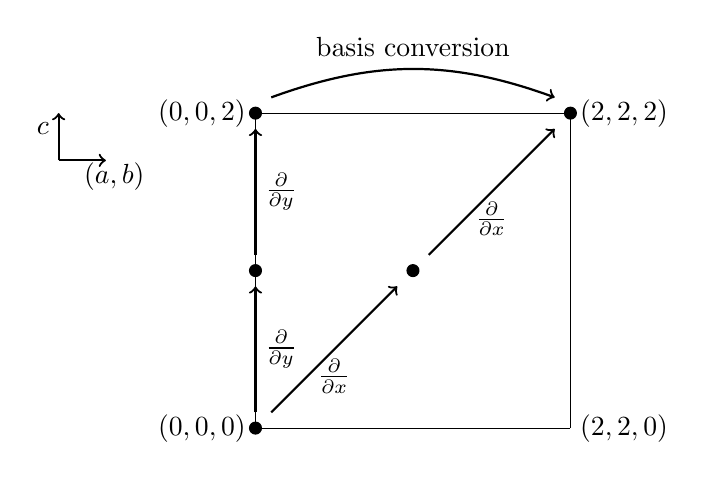
\begin{tikzpicture} 
% Box/square (4x4)
\draw[black,solid,ultra thin] (0,0)--(0,4);
\draw[black,solid,ultra thin] (0,0)--(4,0);
\draw[black,solid,ultra thin] (4,0)--(4,4);
\draw[black,solid,ultra thin] (0,4)--(4,4);
% Dots
\draw[black,fill=black] (0,0) circle (.5ex);
\draw[black,fill=black] (2,2) circle (.5ex);
\draw[black,fill=black] (4,4) circle (.5ex);
\draw[black,fill=black] (0,2) circle (.5ex);
\draw[black,fill=black] (0,4) circle (.5ex);
% Arrows
\draw[black,thick,->] (0.2,0.2)--(1.8,1.8);
\draw[black,thick,->] (2.2,2.2)--(3.8,3.8);
\draw[black,thick,->] (0,0.2)--(0,1.8);
\draw[black,thick,->] (0,2.2)--(0,3.8);
\draw [black,thick,->] (0.2,4.2) to [out=20,in=160] (3.8,4.2);
% Node (parameter) labels
\draw[] (0,0) node[anchor=east] {$(0,0,0)$};
\draw[] (0,4) node[anchor=east] {$(0,0,2)$};
\draw[] (4,0) node[anchor=west] {$(2,2,0)$};
\draw[] (4,4) node[anchor=west] {$(2,2,2)$};
% Arrow labels
\draw[] (1,1) node[anchor=north] {$\tfrac{\partial}{\partial x}$};
\draw[] (3,3) node[anchor=north] {$\tfrac{\partial}{\partial x}$};
\draw[] (0,1) node[anchor=west] {$\tfrac{\partial}{\partial y}$};
\draw[] (0,3) node[anchor=west] {$\tfrac{\partial}{\partial y}$};
% The key and headings
\draw[black,thick,->] (-2.5,3.4)--(-2.5,4);
\draw[black,thick,->] (-2.5,3.4)--(-1.9,3.4);
\draw[] (-2.3,3.2) node[anchor=west] {$(a,b)$};
\draw[] (-2.7,3.6) node[anchor=south] {$c$};
\draw[] (2,4.6) node[anchor=south] {basis conversion};
\end{tikzpicture} 
\caption{The Laplace operator acting on vectors of $\smash{\hdopnk^{(0,0,0)}}$ coefficients has a sparse matrix representation if the range is represented as vectors of $\smash{\hdopnk^{(2,2,2)}}$ coefficients. Here, the arrows indicate that the corresponding operation has a sparse matrix representation when the domain is $\smash{\hdopnkabc}$ coefficients, where $(a,b,c)$ is at the tail of the arrow, and the range is $\smash{\hdopnk^{(\tilde{a},\tilde{b},\tilde{c})}}$ coefficients, where $(\tilde{a},\tilde{b},\tilde{c})$ is at the head of the arrow. %For example, $\smash{\frac{\partial}{\partial x}}$ has a sparse matrix representation when the domain is represented in $\smash{\hdop_{n,k}^{(0,0,0)}}$ (resp.~$\smash{\hdop_{n,k}^{(1,0,1)}}$) and the range in $\smash{\hdop_{n,k}^{(1,0,1)}}$ (resp.~$\smash{\hdop_{n,k}^{(2,0,2)}}$).
}
\label{fig:Laplace} 
\end{figure}


In this section, we will derive the entries that form spherical partial differential operators, demonstrating their sparsity. To this end, we will use a different ordering of the OPs and coefficients of a function's expansion, in order to exploit the orthogonality the circular harmonics will bring and thus the operators will be block-diagonal. Let $N \in \N$ and define: 
\begin{align}
	\bigscopNka &:= 
		\begin{pmatrix}
			\scopa_{k,k,0}(x,y,z) \\
			\scopa_{k,k,1}(x,y,z) \\
			\vdots \\
			\scopa_{N,k,0}(x,y,z) \\
			\scopa_{N,k,1}(x,y,z)
		\end{pmatrix} \in \R^{2(N-k+1)},  \quad k = 1,\dots,N, \label{eqn:OPdefNka} \\ 
	\bigscopa_{N,0} &:= 
		\begin{pmatrix}
			\scopa_{0,0,0}(x,y,z) \\
			\vdots \\
			\scopa_{N,0,0}(x,y,z) \\
		\end{pmatrix} \in \R^{N+1}, \label{eqn:OPdefN0a} \\
	\bigscopNa &:= 
		\begin{pmatrix}
			\bigscopa_{N,0} \\
			\vdots \\
			\bigscopa_{N,N}
		\end{pmatrix} \in \R^{(N+1)^2} \label{eqn:OPdefNa}
\end{align}

We further denote the weighted set of OPs on $\Omega$ by 
\begin{align*}
	\bigWNa(x,y,z) := \genjacw^{(a,0)}(z) \: \bigscopNa(x,y,z),
\end{align*}
and recall that a function $f(x,y,z)$ defined on $\Omega$ is approximated by its expansion $f(x,y,z) = \bigscopa(x,y,z)^\top \mathbf{f}$.

\begin{definition}\label{def:differentialoperators}
Define the operator matrices $D_\phi^{(a)}, \: W_\phi^{(a)}, \: D_\theta, \: \Delta^{(1)}_W$ according to:
\begin{align*}
	\rho {\partial f \over \partial \phi}(x,y,z)&= \bigscop_N^{(a+1)}(x,y,z)^\top \: D_\phi^{(a)} \: \mathbf{f}, \\
	\rho {\partial \over \partial \phi}[\genjacw^{(a,0)}(z) \: f(x,y,z)] &= \bigW_N^{(a-1)}(x,y)^\top \: W_\phi^{(a)}\: \mathbf{f}, \\
	{\partial f \over \partial \theta}(x,y,z) &= \bigscopNa(x,y,z)^\top \: D_\theta \: \mathbf{f}, \\
	\nabla^2_s \big( \genjacw^{(a,0)}(z) \: f(x,y,z) \big) &= \bigscopNa(x,y,z)^\top \: \Delta^{(1)}_W \: \mathbf{f}, \quad \text{ for } a = 1 \text{ only}.
\end{align*}
\end{definition}

The incrementing and decrementing of parameters as seen here is analogous to other well known orthogonal polynomial families' derivatives, for example the Jacobi polynomials on the interval, as seen in the DLMF \cite[(18.9.3)]{DLMF}, on the triangle \cite{olver2018recurrence}, and on the disk-slice \cite{snowball2019sparse}. The operators we define here are for partial derivatives with respect to the spherical coordinates $(\phi, \theta)$, so that we can more easily apply the operators to PDEs on the surface of a sphere (for example, surface Laplacian operator in the Poisson equation).

\begin{theorem}\label{theorem:sparsityofdifferentialoperators}
The operator matrices $D_\phi^{(a)}, \: W_\phi^{(a)}, \: D_\theta, \: \Delta^{(1)}_W$ from Definition \ref{def:differentialoperators} are sparse, with banded-block-banded structure. More specifically:
\begin{itemize}
	\item $D_\phi^{(a)}$ has block-bandwidths $(0,0)$, and sub-block-bandwidths $(2, 4)$
  	\item $W_\phi^{(a)}$ has block-bandwidths $(0,0)$, and sub-block-bandwidths $(4, 2)$
	\item $D_\theta$ has  block-bandwidths $(0,0)$, and sub-block-bandwidths $(1, 1)$
	\item $\Delta^{(1)}_W$ has block-bandwidths $(0,0)$, and sub-block-bandwidths $(1, 1)$
\end{itemize}
\end{theorem}

In order to show the last part of Theorem \ref{theorem:sparsityofdifferentialoperators}, we require the following short Lemma.

\begin{lemma}\label{lemma:Rsecondderivative}
For any general parameter $a$ and any $n = 0,1,\dots$, $k = 0,\dots,n$ we have that
\begin{align*}
	&\ppz[\genjacw^{(a+1, 2(k+1))} \: \genjacnmk^{(a,2k) \: \prime}] \\
	&\quad \quad = \genjacw^{(a+1, 2(k+1))} \: \genjacnmk^{(a,2k) \: \prime \prime} - 2(k+1)z \genjacw^{(a+1, 2k)} \: \genjacnmk^{(a,2k) \: \prime} + (a+1) \genjacw^{(a, 2(k+1))} \: \genjacnmk^{(a,2k) \: \prime} \\
	&\quad \quad = \sum_{m = n-1}^{n+1} \: c_{m,k} \: \genjacw^{(a, 2k)} \: \genjac_{m-k}^{(a,2k)}
\end{align*}
where 
\begin{align*}
	c_{m,k} = - \frac{1}{\normgenjac^{(a,2k)}} \: \int_\alpha^1 \: \genjacnmk^{(a,2k) \: \prime} \: \genjac_{m-k}^{(a,2k) \: \prime} \: \genjacw^{(a+1, 2(k+1))} \: \D z
\end{align*}
\end{lemma}
\begin{proof}[Proof of Lemma \ref{lemma:Rsecondderivative}]
Since $\ppz[\genjacw^{(a+1, 2(k+1))} \: \genjacnmk^{(a,2k) \: \prime}] = \genjacw^{(a, 2k)} \: r_{n-k+1}$ where $r_{n-k+1}$ is a degree $n - k + 1$ polynomial, we have that 
\begin{align*}
	\ppz[\genjacw^{(a+1, 2(k+1))} \: \genjacnmk^{(a,2k) \: \prime}] =\sum_{m=0}^{n-k+1} \: \tilde c_{\{n,k\},m} \: \genjacw^{(a, 2k)} \: \genjac_{m}^{(a,2k)}
\end{align*}
for some coefficients $\tilde c_{\{n,k\},m}$. These coefficients are given by
\begin{align*}
	\tilde c_{\{n,k\},m} &= \frac{1}{\normgenjac^{(a,2k)}} \: \ip<\ppz[\genjacw^{(a+1, 2(k+1))} \: \genjacnmk^{(a,2k) \: \prime}], \genjac_{m}^{(a,2k)}>_{\genjacw^{(0,0)}} \\
	&= - \frac{1}{\normgenjac^{(a,2k)}}  \: \int_\alpha^1 \: \genjacnmk^{(a,2k) \: \prime} \: \genjac_{m}^{(a,2k) \: \prime} \: \genjacw^{(a+1, 2(k+1))} \: \D z
\end{align*}
We show that these are zero for $m < n - k - 1$ by integrating twice by parts:
\begin{align*}
	&\ip<\ppz[\genjacw^{(a+1, 2(k+1))} \: \genjacnmk^{(a,2k) \: \prime}], \genjac_{m}^{(a,2k)}>_{\genjacw^{(0,0)}} \\
	&\quad \quad \quad = - \int_\alpha^1 \: \genjacnmk^{(a,2k) \: \prime} \: \genjac_{m-k}^{(a,2k) \: \prime} \: \genjacw^{(a+1, 2(k+1))} \: \D z \\
	&\quad \quad \quad = \int_\alpha^1 \: \genjacnmk^{(a,2k) \: \prime} \: [(a+1) \genjac_{m}^{(a,2k) \: \prime} \: \genjacw^{(0, 2)} \\
	&\quad \quad \quad \quad \quad \quad \quad \quad \quad \quad - 2(k+1) z \genjac_{m}^{(a,2k) \: \prime} \: \genjacw^{(1, 0)} + \genjac_{m}^{(a,2k) \: \prime \prime} \: \genjacw^{(1, 2)}] \: \genjacw^{(a, 2k)} \: \D z
\end{align*}
which is indeed zero for $m < n - k - 1$ by orthogonality.
\end{proof}

\begin{proof}[Proof of Theorem \ref{theorem:sparsityofdifferentialoperators}]
First, note that:
\begin{align}
	\genjacw^{(a,b) \: \prime}(z) &= a \: \genjacw^{(a-1,b)}(z) + c \: \rho(z) \: \rho'(z) \:\genjacw^{(a,b-2)}(z), \label{eqn:derivativeofweightgenjac} \\
	\rho(z) \: \rho'(z) &= -z \label{eqn:rhoderivative} \\
	{\partial \over \partial \phi} &= -\rho \: {\partial \over \partial z} \label{eqn:partialphitoz} 
\end{align}

For the operator $D_\theta$ for partial differentiation by $\theta$, we simply have that
\begin{align*}
	{\partial \over \partial \theta}\scopnkia(x,y,z) &= \genjacnmk^{(a,2k)}(z) \: \rho(z)^{k} \: {\partial \over \partial \theta} \chki(\theta) \\
	&= 
	\begin{cases}
		(-1)^{i+1} \: k \: \scopa_{n,k,|i-1|}(x,y,z) & k > 0 \\
		0 & k = 0
	\end{cases}
\end{align*}

We now proceed with the case for the operator $D_\phi^{(a)}$ for partial differentiation by $\phi$. The entries of the operator are given by the coefficients in the expansion $\rhoppphi \scopnkia = \sum_{m=0}^{n+1} \sum_{j=0}^m \sum_{h=0}^1 c_{m,j,h} \: \scopmjh^{(a+1)}$, where the coefficients are
\begin{align*}
	c_{m,j,h} = \norm{\scopmjh^{(a+1)}}^{-2}_{\scop^{(a+1)}} \ip<\rhoppphi \scopnkia, \: \scopmjh^{(a+1)}>_{\scop^{(a+1)}}.
\end{align*}
Now,
\begin{align*}
	&\ip<\rhoppphi \scopnkia, \: \scopmjh^{(a+1)}>_{\scop^{(a+1)}} \\
	&\quad = - \int_\Omega \: \rho(z)^2 \ppz \:  [\genjacnmk^{(a,2k)}(z) \: \rho(z)^k] \: \genjacmmj^{(a+1,2j)}(z) \: \rho(z)^j \: \chki(\theta) \: \chjh(\theta) \: \genjacw^{(a+1, 0)} \: \D \Omega \\
	&\quad = \Big( \int_0^{2\pi} \: \chki(\theta) \: \chjh(\theta) \: \D \theta \Big) \: \Big( \int_\alpha^1 \: \genjacmmj^{(a+1,2j)} \: [k z \genjacnmk^{(a, 2k)} - \rho^2 \genjacnmk^{(a, 2k) \: \prime}] \: \genjacw^{(a+1, k + j)} \: \D z \Big) \\
	&\quad = \pi \: \delta_{k,j} \: \delta_{i,h} \: \int_\alpha^1 \: \genjac_{m-k}^{(a+1,2k)} \: [k z \genjacnmk^{(a, 2k)} - \rho^2 \genjacnmk^{(a, 2k) \: \prime}] \: \genjacw^{(a+1, 2k)} \: \D z \\
	&\quad = \pi \: \delta_{k,j} \: \delta_{i,h} \: \int_\alpha^1 \: \genjacnmk^{(a, 2k)} \: \Big\{  k z \: \genjac_{m-k}^{(a+1,2k)} \: \genjacw^{(1, 0)} + \genjac_{m-k}^{(a+1,2k) \: \prime} \: \genjacw^{(1, 2)}\\
	&\quad \quad \quad \quad \quad \quad \quad \quad \quad \quad \quad \quad \quad + a \: \rho^2 \: \genjac_{m-k}^{(a+1,2k)} - (2k+2) z \: \genjac_{m-k}^{(a+1,2k)} \: \genjacw^{(1, 0)} \Big\} \: \genjacw^{(a, 2k)} \: \D z
\end{align*}
which is zero for $j \ne k$, $h \ne i$, and $m < n - 2$ by orthogonality.

Similarly for the operator $W_\phi^{(a)}$ for partial differentiation by $\phi$ on the weighted space, the entries of the operator are given by the coefficients in the expansion $\rhoppphi (\genjacw^{(a,0)} \: \scopnkia) = \sum_{m=0}^{n+2} \sum_{j=0}^m \sum_{h=0}^1 c_{m,j,h} \: \genjacw^{(a-1,0)} \: \scopmjh^{(a-1)}$, where the coefficients are
\begin{align*}
	c_{m,j,h} = \norm{\scopmjh^{(a-1)}}^{-2}_{\scop^{(a-1)}} \ip<\rhoppphi (\genjacw^{(a,0)} \: \scopnkia), \: \scopmjh^{(a-1)}>_{\scop^{(0)}}.
\end{align*}
Now,
\begin{align*}
	&\ip<\rhoppphi (\genjacw^{(a,0)} \: \scopnkia), \: \scopmjh^{(a-1)}>_{\scop^{(0)}} \\
	&\quad = - \int_\Omega \: \rho(z)^2 \ppz \:  [\genjacnmk^{(a,2k)}(z) \: \rho(z)^k \: \genjacw^{(a, 0)}(z)] \: \genjacmmj^{(a-1,2j)}(z) \: \rho(z)^j \: \chki(\theta) \: \chjh(\theta) \: \D \Omega \\
	&\quad = \Big( \int_0^{2\pi} \: \chki(\theta) \: \chjh(\theta) \: \D \theta \Big) \\
	&\quad \quad \quad \quad \cdot \: \Big( \int_\alpha^1 \: \genjacmmj^{(a-1,2j)} \: [k z \genjacnmk^{(a, 2k)} \: \genjacw^{(1, 0)} - \genjacnmk^{(a, 2k) \: \prime} \: \genjacw^{(1, 2)} - a \: \genjacnmk^{(a, 2k)} \: \rho^2] \: \genjacw^{(a-1, k + j)} \: \D z \Big) \\
	&\quad = \pi \: \delta_{k,j} \: \delta_{i,h} \:  \int_\alpha^1 \: \genjac_{m-k}^{(a-1,2k)} \: [k z \genjacnmk^{(a, 2k)} \: \genjacw^{(1, 0)} - \genjacnmk^{(a, 2k) \: \prime} \: \genjacw^{(1, 2)} - a \: \genjacnmk^{(a, 2k)} \: \rho^2] \: \genjacw^{(a-1, 2k)} \: \D z \\
	&\quad = \pi \: \delta_{k,j} \: \delta_{i,h} \: \int_\alpha^1 \: \genjacnmk^{(a, 2k)} \: \Big\{  k z \: \genjac_{m-k}^{(a-1,2k)} \: \genjacw^{(1, 0)} - a \: \rho^2 \: \genjac_{m-k}^{(a-1,2k)} + \genjac_{m-k}^{(a-1,2k) \: \prime} \: \genjacw^{(1, 2)} \\
	&\quad \quad \quad \quad \quad \quad \quad \quad \quad \quad \quad \quad \quad + a \: \rho^2 \: \genjac_{m-k}^{(a-1,2k)} - (2k+2) z \: \genjac_{m-k}^{(a-1,2k)} \: \genjacw^{(1, 0)} \Big\} \: \genjacw^{(a-1, 2k)} \: \D z \\
	&\quad = \pi \: \delta_{k,j} \: \delta_{i,h} \: \int_\alpha^1 \: \genjacnmk^{(a, 2k)} \: \Big\{  k z \: \genjac_{m-k}^{(a-1,2k)} + \genjac_{m-k}^{(a-1,2k) \: \prime} \: \rho^2- (2k+2) z \: \genjac_{m-k}^{(a-1,2k)} \Big\} \: \genjacw^{(a, 2k)} \: \D z
\end{align*}
which is zero for $j \ne k$, $h \ne i$, and $m < n - 1$ by orthogonality.

Finally, fix $a = 1$. For the operator $\Delta^{(1)}_W$ for the Laplacian on the weighted space, the entries of the operator are given by the coefficients in the expansion $\nabla^2_s \big(\genjacw^{(1,0)} \: \scopnki^{(1)} \big) = \sum_{m=0}^{n+2} \sum_{j=0}^m \sum_{h=0}^1 c_{m,j,h} \: \scopmjh^{(1)}$, where the coefficients are
\begin{align*}
	c_{m,j,h} = \norm{\scopmjh^{(1)}}^{-2}_{\scop^{(1)}} \ip<\nabla^2_s \big(\genjacw^{(1,0)} \: \scopnki^{(1)} \big), \: \scopmjh^{(1)}>_{\scop^{(1)}}.
\end{align*}
Now, note that the Laplacian acting on the weighted spherical cap OP $\scopnki^{(a)}$ yields
\begin{align*}
	\nabla^2_s \big(\genjacw^{(1,0)} \: \scopnki^{(1)} \big) &= 
\end{align*}
Hence,
\begin{align*}
	&\ip<\nabla^2_s \big(\genjacw^{(1,0)} \: \scopnki^{(1)} \big), \: \scopmjh^{(1)}>_{\scop^{(1)}} \\
	&\quad = \Big( \int_0^{2\pi} \: \chki(\theta) \: \chjh(\theta) \: \D \theta \Big) \\
	&\quad \quad \quad \quad \cdot \: \Big( \int_\alpha^1 \: \genjacmmj^{(1,2j)} \: \Big\{ \genjacnmk^{(a, 2k)} \: [- k^2 \genjacw^{(1, k)} - \genjacw^{(1, k)} - 2(k + 1)z \genjacw^{(0, k)}] \\
	&\quad \quad \quad \quad \quad \quad \quad \quad \quad \quad \quad \quad + \genjacnmk^{(a, 2k) \: \prime} \: [2 \genjacw^{(0, k+2)} - 2(k + 1)z \genjacw^{(1, k)}] \\
	&\quad \quad \quad \quad \quad \quad \quad \quad \quad \quad \quad \quad + \genjacnmk^{(a, 2k) \: \prime \prime} \: \genjacw^{(1, k+2)} \Big\} \: \genjacw^{(1, j)} \: \D z \Big) \\
	&\quad = \pi \: \delta_{k,j} \: \delta_{i,h} \: \int_\alpha^1 \: \genjac_{m-k}^{(1,2k)} \: \Big\{ \genjacnmk^{(a, 2k)} [-k(k+1) \genjacw^{(1, 0)} - 2(k+1)z + c_{n,k}] \\
	&\quad \quad \quad \quad \quad \quad \quad \quad \quad \quad \quad \quad + c_{n-1,k} \genjac_{n-k-1}^{(a, 2k)} + c_{n+1,k} \genjac_{n-k+1}^{(a, 2k)} \Big\} \: \genjacw^{(1, 2k)} \: \D z \\
	&\quad = - \pi \: \delta_{k,j} \: \delta_{i,h} (\delta_{m,n-1} + \delta_{m,n} + \delta_{m,n+1}) \: \int_\alpha^1 \: \Big\{ \genjac_{m-k}^{(1,2k)} \: \genjacnmk^{(a, 2k)} (k(k+1) \genjacw^{(1, 0)} + 2(k+1)z) \\ 
	&\quad \quad \quad \quad \quad \quad \quad \quad \quad \quad \quad \quad \quad \quad \quad \quad \quad \quad \quad \quad \quad + \genjacnmk^{(a,2k) \: \prime} \: \genjac_{m-k}^{(a,2k) \: \prime} \: \genjacw^{(a+1, 2(k+1))} \Big\} \: \D z
\end{align*}
where the $c_{n-1,k}, c_{n,k}, c_{n+1,k}$ are those derived in Lemma \ref{lemma:Rsecondderivative}.
\end{proof}

There exist conversion matrix operators that increment/decrement the parameters, transforming the OPs from one (weighted or non-weighted) parameter space to another. 

\begin{definition}\label{def:parametertransformationoperators}
Define the operator matrices $T^{(a)\to(a+\tilde a)}, \quad T^{(a)\to(a-\tilde a)}$ for conversion between non-weighted spaces and weighted spaces respectively according to
\begin{align*}
	\bigscopNa(x,y,z) &= \Big(T^{(a)\to(a+\tilde a)} \Big)^\top \: \bigscopN^{(a+\tilde a)}(x,y,z) \\
	\bigWNa(x,y,z) &= \Big(T_W^{(a)\to(a-\tilde a)} \Big)^\top \: \bigW_N^{(a-\tilde a)}(x,y,z)
\end{align*}
\end{definition}

\begin{lemma}\label{lemma:sparsityofparametertransformationoperators}
The operator matrices in Definition \ref{def:parametertransformationoperators} are sparse, with banded-block-banded structure. More specifically:
\begin{itemize}
	\item $T^{(a)\to(a+\tilde a)}$ is block-diagonal with sub-block bandwidths $(0,2\tilde a)$
	\item $T_W^{(a)\to(a-\tilde a)}$ is block-diagonal with sub-block bandwidths $(2\tilde a, 0)$
\end{itemize}
\end{lemma}

\begin{proof}
We proceed with the case for the non-weighted operators $T^{(a)\to(a+\tilde a)}$. Since $\{\scopmjh^{(a+\tilde{a})}\}$ for $m = 0,\dots,n$, $j = 0,\dots,m$, $h = 0,1$ is an orthogonal basis for any degree $n$ polynomial, we can expand $\scopnkia = \sum_{m=0}^{n} \sum_{j=0}^m t_{m,j} \: \scopmjh^{(a+\tilde{a})}$. The coefficients of the expansion are then the entries of the operator matrix. We will show that the only non-zero coefficients are for $k = j$, $i = h$ and $m \ge  n - \tilde a$. Note that
\begin{align*}
	t_{m,j} = \norm{\scopmjh^{(a+\tilde{a})}}^{-2}_{\scop^{(a+\tilde a)}} \: \ip< \scopnkia, \scopmjh^{(a+\tilde{a})}>_{\scop^{(a+\tilde a)}}.
\end{align*}
where
\begin{align*}
	\ip< \scopnkia, \scopmjh^{(a+\tilde{a})}>_{\scop^{(a+\tilde a)}} &= \Big( \int_0^{2\pi} \: \chki(\theta) \: \chjh(\theta) \: \D \theta \Big) \: \cdot \: \Big( \int_\alpha^1 \: \genjacnmk^{(a, 2k)} \: \genjacmmj^{(a+\tilde a,2j)} \: \rho^{k+j} \: \genjacw^{(a + \tilde a, 0)} \: \D z \Big) \\
	&= \pi \: \delta_{k,j} \: \delta_{i,h} \: \int_\alpha^1 \: \genjacnmk^{(a, 2k)} \: \genjac_{m-k}^{(a+\tilde a,2k)} \: \genjacw^{(a + \tilde a, 2k)} \: \D z
\end{align*}
which is zero for $n > m + \tilde a \iff m < n - \tilde a$. The sparsity argument for the weighted parameter transformation operator follows similarly.
\end{proof}

\begin{figure}[t]
	\begin{subfigure}{0.32\textwidth}
	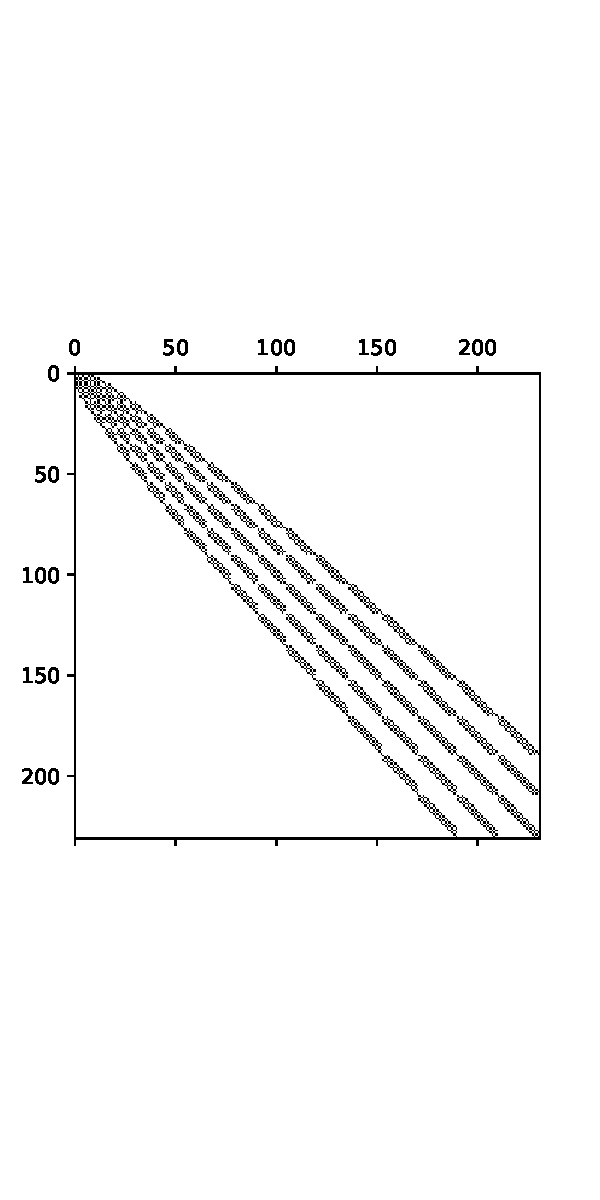
\includegraphics[scale=0.35]{sparsityoflaplacian-w11-diskslice-alpha=0p2-beta=0p8}
        \centering
	\end{subfigure}
	\begin{subfigure}{0.32\textwidth}
	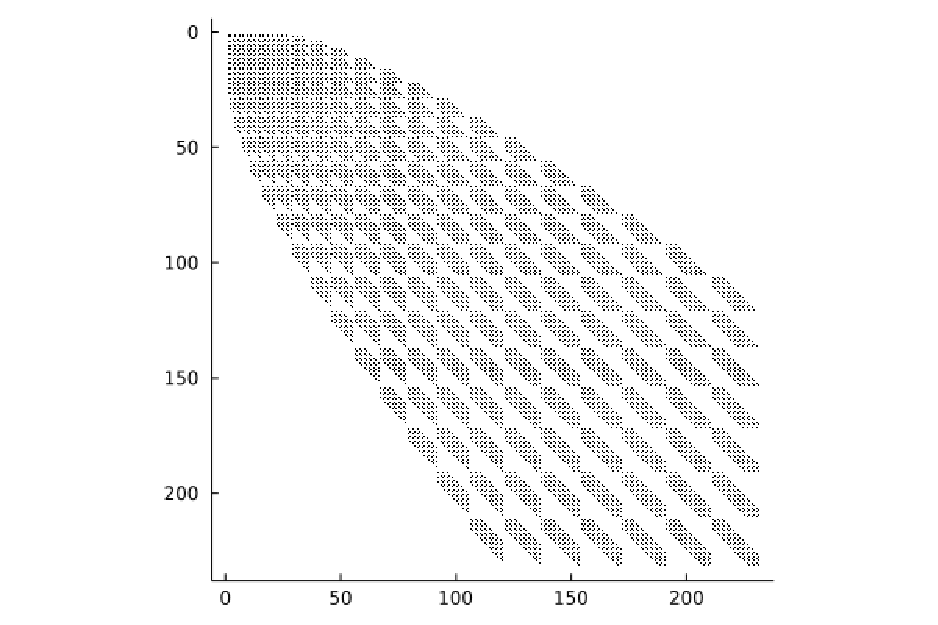
\includegraphics[scale=0.35]{sparsityofhelmholtz-diskslice-alpha=0p2-beta=0p8}
        \centering
	\end{subfigure}
	\begin{subfigure}{0.32\textwidth}
	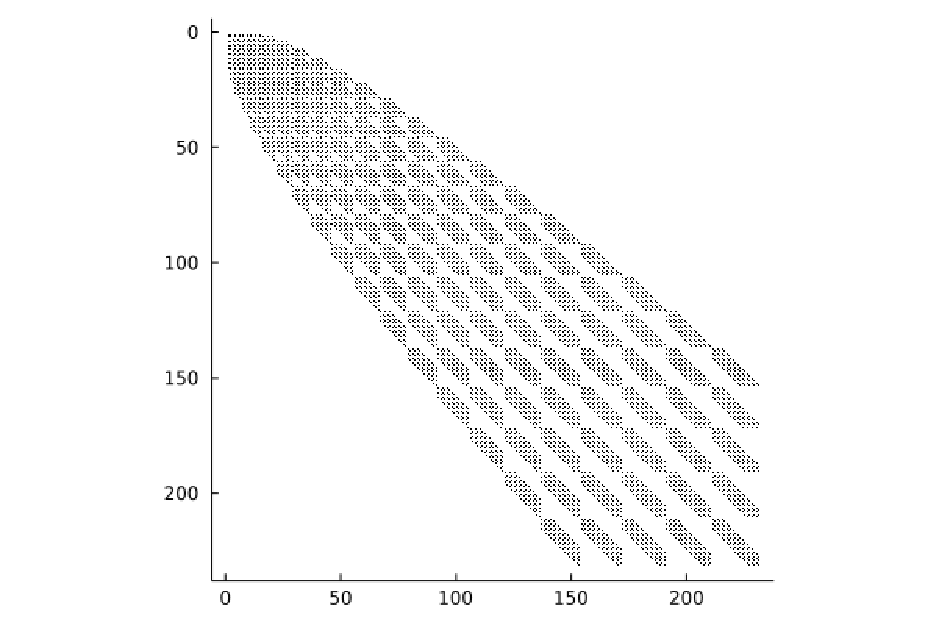
\includegraphics[scale=0.35]{sparsityofbiharmonic-diskslice-alpha=0p2-beta=0p8}
        \centering
	\end{subfigure}
    	\caption{"Spy" plots of (differential) operator matrices, showing their sparsity. Left: the Laplace operator $\laplacewiii$. Centre: the weighted variable coefficient Helmholtz operator $\laplacewiii + k^2 \: T^{(0,0,0)\to(1,1,1)} \: V({J_x^{(0,0,0)}}^\top, {J_y^{(0,0,0)}}^\top) \: T_W^{(1,1,1)\to(0,0,0)}$ for $v(x,y) = 1 - (3(x-1)^2 + 5y^2)$ and $k = 200$. Right: the biharmonic operator $\biharmonictwo$.}
        \label{fig:sparsity}
        \centering
\end{figure}

General linear partial differential operators with polynomial variable coefficients can be constructed by composing the sparse representations for partial derivatives, conversion between bases, and Jacobi operators. As a canonical example, we can obtain the matrix operator for the $\rho^2$-factored surface Laplacian $\rho(z)^2 \: \nabla^2_s$, that will take us from coefficients for expansion in the weighted space
$$
\bigW_N^{(1)}(x,y,z) = \genjacw^{(1,0)}(z) \: \bigscopN^{(1)}(x,y,z)
$$
to coefficients in the non-weighted space $\bigscopN^{(1)}(x,y,z)$. Note that this construction will ensure the imposition of the Dirichlet zero boundary conditions on $\Omega$, similar to how the Dirichlet zero boundary conditions would be imposed for the operator $\Delta^{(1)}_W$ in Definition \ref{def:differentialoperators}. The matrix operator for this $\rho^2$-factored Laplacian we denote $\mathcal{L}_W^{(1)}$ acting on the coefficients vector is then given by
\begin{align*}
    \mathcal{L}_W^{(1)} := D_\phi^{(0)} \: W_\phi^{(1)} + T^{(0)\to(1)} \: T_W^{(1)\to(0)} \: (D_\theta)^2.
\end{align*}
Importantly, this operator will have banded-block-banded structure, and hence will be sparse, as seen in Figure \ref{fig:sparsity}.

Another important example is the Biharmonic operator $\Delta^2_s$ (defined by $\Delta^2_s f = \nabla^2_s (\nabla^2_s f)$), where we assume zero Dirichlet and Neumann conditions. To construct an operator for the Biharmonic function, we first note that we can obtain the matrix operator for the $\rho^2$-factored Laplacian $\rho(z)^2 \: \nabla^2_s$ that will take us from coefficients for expansion in the space $\bigscopN^{(0)}(x,y,z)$ to coefficients in the space $\bigscopN^{(2)}(x,y,z)$. We denote this matrix operator that acts on the coefficients vector as $\mathcal{L}^{(0) \to (2)}$, and is given by
\begin{align*}
    \mathcal{L}^{(0) \to (2)} := D_\phi^{(2)} \: D_\phi^{(0)} + T^{(0)\to(2)} \: D_\theta.
\end{align*}
Further, we can represent this same Laplacian as a map from coefficients in the space $\bigW_N^{(2)}$ to coefficients in the space $\bigW_N^{(0)} \equiv \bigscopN^{(0)}$. Note that a function expanded in the $\bigW_N^{(2)}$ basis will satisfy both zero Dirichlet and Neumann boundary conditions on $\Omega$. We denote this matrix operator as $\mathcal{L}_W^{(2) \to (0)}$, and is given by
\begin{align*}
	\mathcal{L}_W^{(2) \to (0)} := W_\phi^{(1)} \: W_\phi^{(2)} + T_W^{(2)\to(0,0,0)} \: D_\theta.
\end{align*}
We can then construct a matrix operator for $\Delta^2_s$ that will take coefficients in the space $\bigW_N^{(2)}$ to coefficients in the space $\bigscopN^{(2)}$. Note that any function expanded in the $\bigW_N^{(2)}$ basis will satisfy both zero Dirichlet and zero Neumann boundary conditions on $\Omega$. Since, for any scalar function $f:\Omega \to \R$,
\begin{align*}
	\rho^2(z) \: \Delta^2 \: f(x,y,z) = \rho^2 \: \nabla^2_s (\rho^2 \: \nabla^2_s f) - z \: \rhoppphi (\rho^2 \: \nabla^2_s f) - [2z^2 - 2\rho^2 + 3z] \:\rho^2 \: \nabla^2_s f
\end{align*}
the matrix operator for the $\rho^2$-factored Biharmonic operator $\rho(z)^2 \: \Delta_s^2$ is then given by
\begin{align*}
	\mathcal{B}_W^{(2)} := \mathcal{L}^{(0) \to (2)} \: \mathcal{L}_W^{(2) \to (0)} - (J_z^{(2)})^\top \: T^{(1)\to(2)} \: D_\phi^{(0)} \: \mathcal{L}_W^{(2) \to (0)} - V^{(2)} \:  T^{(0)\to(2)} \: \mathcal{L}_W^{(2) \to (0)},
\end{align*}
where $V^{(a)}$ is an operator corresponding to multiplication by the scalar function $v(z) := 2z^2 - 2\rho(z)^2 + 3z = 4z^2 + 3z - 2$ acting on coefficients in the $\bigscopN^{(a)}$ space.
The sparsity and structure of this biharmonic operator are seen in Figure \ref{fig:sparsity}.



%
\section{Computational aspects}\label{Section:Computation}

In this section we discuss how to take advantage of the proposed basis and sparsity structure in partial differential operators in practical computational applications.

\subsection{Constructing $\genjac_n^{(a,b)}(x)$}

It is possible to recursively obtain the recurrence coefficients for the $\{\genjac_n^{(a,b)}\}$ OPs in (\ref{eqn:Rrecurrence}), see \cite{snowball2019sparse}, by careful application of the Christoffel--Darboux formula \cite[18.2.12]{DLMF}.

\subsection{Quadrature rule on the spherical cap}\label{subsection:quadrule}

In this section we construct a quadrature rule exact for polynomials on the spherical cap $\Omega$ that can be used to expand functions in the OPs $\scopnkia(x,y,z)$ for a given parameter $a$.

\begin{theorem}\label{Theorem:quadrule}
Let $M_1, M_2 \in \N$ and denote the $M_1$ Gauss quadrature nodes and weights on $[\alpha,1]$ with weight $(t - \alpha)^a$ as $(t_j, w_j^{(t)})$. Further, we denote the $M_2$ Gauss quadrature nodes and weights for the unit circle \cite{???}\bstodo{good reference?} by $(\mathbf{s}_j, w_j^{(s)})$ where for $j = 1,\dots,M_2$:
\begin{align*}
	\mathbf{s}_j &= \Big( \cos\fpr(\frac{2 \pi j}{M_2}), \: \sin\fpr(\frac{2 \pi j}{M_2}) \Big), \\
	w_j^{(s)} &= \frac{2\pi}{M_2}.
\end{align*}
Define for $j = 1,\dots,M_1, \: l=1,\dots,M_2$:
\begin{align*}
	\big(x_{l+(j-1)M_2}, \: y_{l+(j-1)M_2} \big) &:= \rho(t_j) \: \mathbf{s}_l, \\
	z_{l+(j-1)M_2} &:= t_j, \\
	w_{l+(j-1)M_2} &:= w_j^{(t)} w_l^{(s)}.
\end{align*}
Let $f(x,y,z)$ be a function on $\Omega$, and $N \in \N$. The quadrature rule is then
\begin{align*}
	\int_\Omega f(x,y,z) \: \genjacw^{(a,0)}(z) \: \D \sigma(x,y) \: \D z \approx \half \sum_{j=1}^{M} w_j \: \big[ f(x_j, y_j, z_j) + f(-x_j, -y_j, z_j) \big],
\end{align*}
where $M = M_1 \: M_2$, and the quadrature rule is exact if $f(x,y,z)$ is a polynomial of degree $\le N$ with $M_1 \ge \half (N+1), M_2 \ge N+1$.
\end{theorem}

\begin{proof}
Let $f : \Omega \to \R$. Define the functions $f_e, f_o : \Omega \to \R$ by 
\begin{align*}
	f_e(x,y,z) &:= \half \Big(f(x, y,z) + f(-x, -y,z)\Big), \quad \forall (x,y,z) \in \Omega\\
	f_o(x,y,z) &:= \half \Big(f(x, y,z) - f(-x, -y,z)\Big), \quad \forall (x,y,z) \in \Omega
\end{align*}
so that $\xvec \mapsto f_e(\xvec, z)$ for fixed $z$ is an even function, and $\xvec \mapsto f_o(\xvec, z)$ for fixed $z$ is an odd function. Note that if $f$ is a polynomial, then $f_e(\rho(t)\xvec, t)$ is a polynomial in $t \in [\alpha,1]$ for fixed $\xvec \in \R^2$. 

Now, we have that
\begin{align*}
	&\int_\Omega f_e(x,y,z) \: \genjacw^{(a,0)}(z) \: \D \sigma(x,y) \: \D z \\
	&\quad \quad = \int_0^{\cos^{-1}(\alpha)} \int_0^{2\pi} f_e\big(\cos(\theta)\sin(\phi), \sin(\theta)\sin(\phi), \cos(\phi)\big) \: \genjacw^{(a,0)}\big(\cos(\phi)\big) \: \sin(\phi) \: \D \theta \: \D \phi \\
	&\quad \quad = \int_\alpha^1 \genjacw^{(a,0)}(z) \: \Big( \int_0^{2\pi} f_e\big(\rho(z)\cos(\theta),\rho(z)\sin(\theta), z)\big) \: \D \theta \Big) \: \D z \\
	&\quad \quad = \int_\alpha^1 \genjacw^{(a,0)}(z) \: \Big( \int_{\norm{\mathbf{\xi}} = 1} f_e\big(\rho(z)\mathbf{\xi}, z)\big) \: \D \sigma(\mathbf{\xi}) \Big) \: \D z \\
	&\quad \quad \approx\int_\alpha^1 \genjacw^{(a,0)}(z) \: \Big( \sum_{l=1}^{M_2} w_l^{(s)} f_e\big(\rho(z) \mathbf{s}_l, z\big) \Big) \: \D z \quad (\star) \\
	&\quad \quad \approx \sum_{j=1}^{M_1} w_j^{(t)} \sum_{l=1}^{M_2} w_l^{(s)} f_e\big(\rho(t_j) \mathbf{s}_l, t_j\big) \quad (\star \star) \\
	&\quad \quad = \sum_{k=1}^{M_1 M_2}  w_j \: f_e(x_j, y_j, z_j).
\end{align*}
Suppose $f$ is a polynomial in $x,y,z$ of degree $N$, and hence that $f_e$ is a degree $\le N$ polynomial. We therefore achieve equality at $(\star)$ if $M_2 - 1 \ge N$ and we achieve equality at $(\star \star)$ if also $2M_1 - 1 \ge N$. \bstodo{For the circle rule, is this bound on N true?}

Next, note that 
\begin{align*}
	&\int_\Omega f_o(x,y,z) \: \genjacw^{(a,0)}(z) \: \D \sigma(x,y) \: \D z \\
	&\quad \quad = \int_0^{\cos^{-1}(\alpha)} \int_0^{2\pi} f_o\big(\cos(\theta)\sin(\phi), \sin(\theta)\sin(\phi), \cos(\phi)\big) \: \genjacw^{(a,0)}\big(\cos(\phi)\big) \: \sin(\phi) \: \D \theta \: \D \phi \\
	&\quad \quad = \int_\alpha^1 \genjacw^{(a,0)}(z) \: \Big( \int_0^{2\pi} f_o\big(\rho(z)\cos(\theta),\rho(z)\sin(\theta), z)\big) \: \D \theta \Big) \: \D z \\
	&\quad \quad = \int_\alpha^1 \genjacw^{(a,0)}(z) \: \Big( \int_{\norm{\mathbf{\xi}} = 1} f_o\big(\rho(z)\mathbf{\xi}, z)\big) \: \D \sigma(\mathbf{\xi}) \Big) \: \D z \quad (\dagger) \\
	&\quad \quad = 0
\end{align*}
since the inner integral at $(\dagger)$ over $\mathbf{\xi}$ is zero, due to the symmetry over the domain.

Hence, for a polynomial $f$ in $x,y,z$ of degree $N$,
\begin{align*}
	\int_\Omega f(x,y,z) \: \genjacw^{(a,0)}(z) \: \D \sigma(x,y) \: \D z &= \int_\Omega \Big(f_e(x,y,z) + f_o(x,y,z)\Big) \:  \genjacw^{(a,0)}(z) \: \D \sigma(x,y) \: \D z  \\
	&= \int_\Omega f_e(x,y,z) \: \genjacw^{(a,0)}(z) \: \D \sigma(x,y) \: \D z \\
	&= \sum_{j=1}^{M}  w_j \: f_e(x_j, y_j, z_j),
\end{align*}
where $M = M_1 M_2$ and $2M_1 - 1 \ge N, M_2 - 1 \ge N$.
\end{proof}


\subsection{Obtaining the coefficients for expansion of a function on the spherical cap}\label{subsection:expandingfunctions}

Fix $a \in \R$. Then for any function $f : \Omega \to \R$ we can express $f$ by
\begin{align*}
	f(x,y,z) \approx \sum_{k=0}^N \bigscopNka(x,y,z)^\top \: \mathbf{f}_k
\end{align*}
for N sufficiently large, where $\bigscopNka$ is defined in equation \label{eqn:OPdefNka} and where
\begin{align*}
	\mathbf{f}_k &:= 
		\begin{pmatrix}
			f_{k,k,0} \\
			f_{k,k,1} \\
			\vdots \\
			f_{N,k,0} \\
			f_{N,k,1}
		\end{pmatrix} \in \R^{2(N-k+1)} \quad \text{for } n = 1,2,\dots,N, \quad
	\mathbf{f}_0 := 
		\begin{pmatrix}
			f_{0,0,0} \\
			\vdots \\
			f_{N,0,0}
		\end{pmatrix} \in \R^{2(N+1)},
\end{align*}
\begin{align*}
	f_{n,k,i} &:= \ip< f, \: \scopnkia>_{\scopa} \: \norm{\scopnkia}^{-2}_{\scopa}.
\end{align*}
Recall from (\ref{eqn:OPnorm}) that $\norm{\scopnkia}^2_{\scopa} = \normgenjac^{(a,2k)} \: \pi$. Using the quadrature rule detailed in Section \ref{subsection:quadrule} for the inner product, we can calculate the coefficients $f_{n,k,i}$ for each $n = 0,\dots,N$, $k = 0,\dots,n$, $i = 0,1$: 
\begin{align*}
	f_{n,k,i} &= \frac{1}{2 \: \normgenjac^{(a,2k)} \: \pi} \sum_{j=1}^{M} w_j \big[ f(x_j, y_j, z_j) \scopnkia(x_j, y_j, z_j) +f(-x_j, -y_j, z_j) \scopnkia(-x_j, -y_j, z_j) \big] \\
	&= \frac{1}{M_2 \: \normgenjac^{(a,2k)}} \sum_{j=1}^{M} \big[ f(x_j, y_j, z_j) \scopnkia(x_j, y_j, z_j) +f(-x_j, -y_j, z_j) \scopnkia(-x_j, -y_j, z_j) \big]
\end{align*}
where the quadrature nodes and weights are those from Theorem \ref{Theorem:quadrule}, and $M = M_1 M_2$ with $2M_1 - 1 \ge N, M_2 - 1 \ge N$ (i.e. we can choose $M_2 := N + 1$ and $M_1 := \ceil{\frac{N+1}{2}}$).


\subsection{Calculating non-zero entries of the operator matrices}\label{subsection:Computation-operatormatrices}

The proofs of Theorem \ref{theorem:sparsityofdifferentialoperators} and Lemma \ref{lemma:sparsityofparametertransformationoperators} provide a way to calculate the non-zero entries of the operator matrices given in Definition \ref{def:differentialoperators} and Definition \ref{def:parametertransformationoperators}. We can simply use quadrature to calculate the 1D inner products, which has a complexity of $\bigO(N^3)$. This proves much cheaper computationally than using the 3D quadrature rule to calculate the 3D inner products, which has a complexity of $\bigO(N^4)$ \bstodo{correct the O(nd) complexity}. 


%
\section{Examples on the disk-slice with zero Dirichlet conditions}\label{Section:Examples}

We now demonstrate how the sparse linear systems constructed as above can be used to efficiently solve PDEs with zero Dirichlet conditions on the spherical cap defined by $\Omega$. We consider Poisson, inhomogeneous variable coefficient Helmholtz equation and the Biharmonic equation, as well as a time dependent heat equation, demonstrating the versatility of the approach.

\subsection{Poisson}

% FIGURES
\begin{figure}[t]
	\begin{subfigure}{0.3\textwidth}
	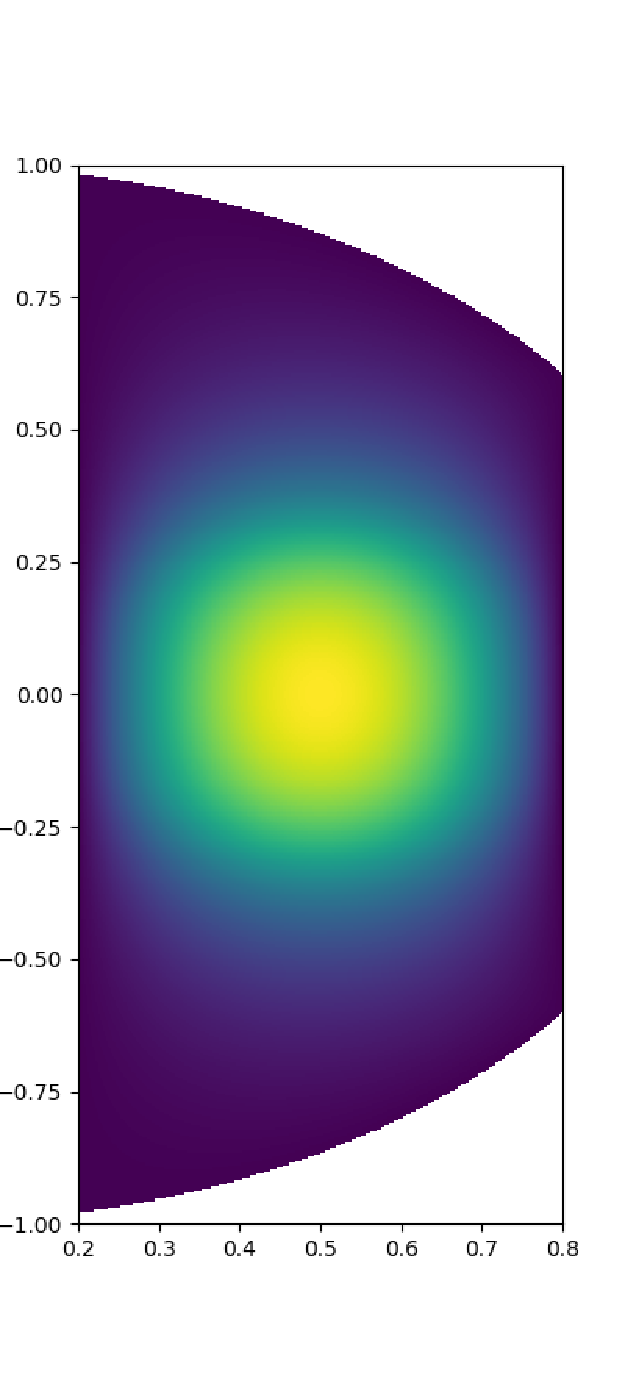
\includegraphics[scale=0.3]{solution-poisson-diskslice-alpha=0p2-beta=0p8}
	\centering
	%\label{fig:solution-poisson}
	\end{subfigure}
	\begin{subfigure}{0.5\textwidth}
	\centering
	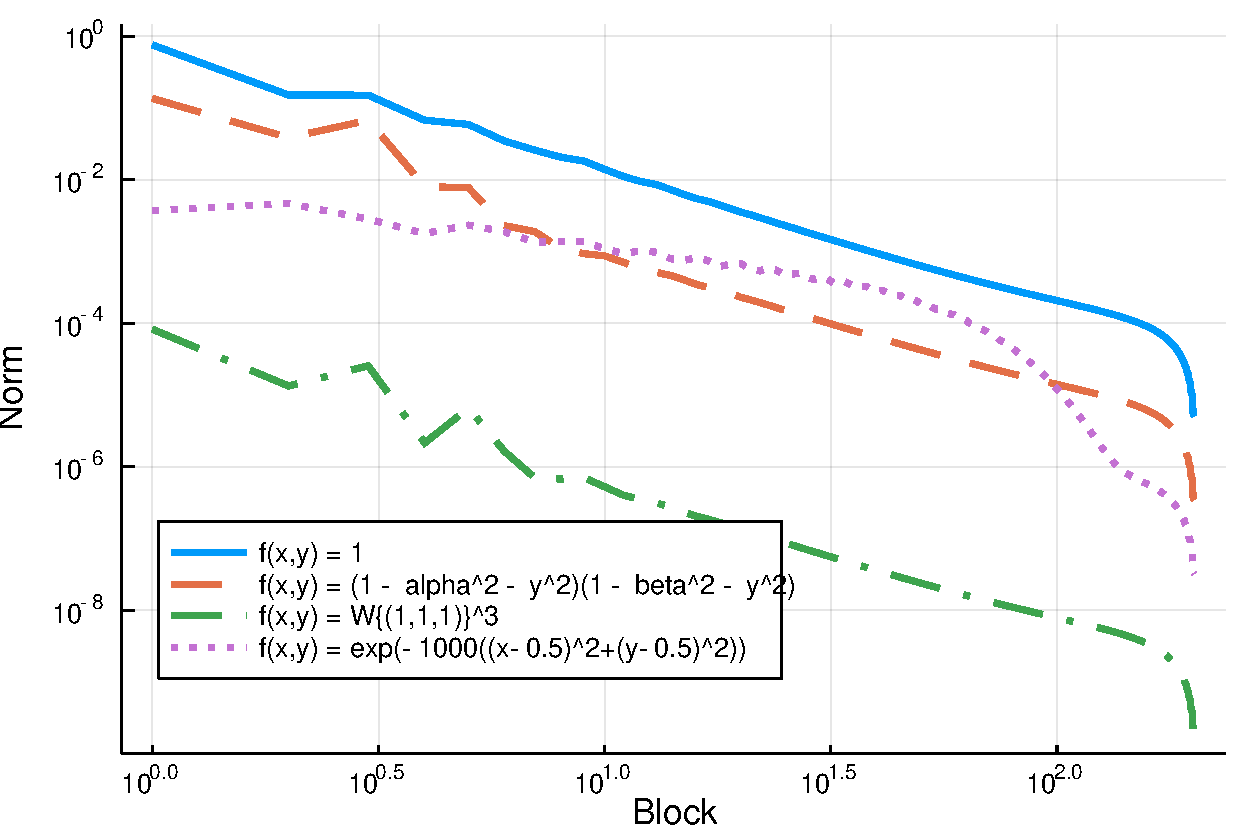
\includegraphics[scale=0.5]{solutionblocknorms-poisson-diskslice-alpha=0p2-beta=0p8-N=200}
        	%\label{fig:solutionblocknorms-poisson}
	\end{subfigure}
	\caption{Left: The computed solution to $\Delta u = f$ with zero boundary conditions with $f(x,y) = 1 + \text{erf}(5(1 - 10((x - 0.5)^2 + y^2)))$. Right: The norms of each block of the computed solution of the Poisson equation with the given right hand side functions. This demonstrates algebraic convergence with the rate dictated by the decay at the corners, with spectral convergence observed when the right-hand side vanishes to all orders.}
	\centering
	\label{fig:poisson}
\end{figure}

\begin{figure}[t]
	\begin{subfigure}{0.3\textwidth}
	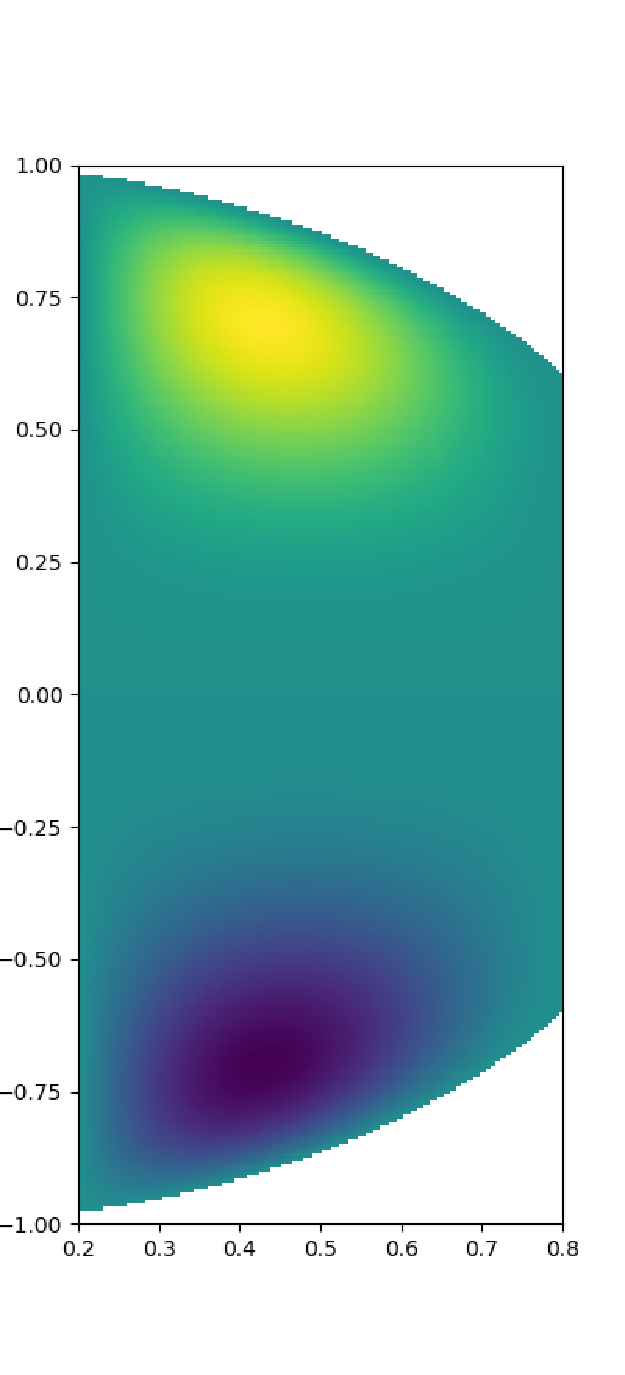
\includegraphics[scale=0.3]{solution-exact-poisson-diskslice-alpha=0p2-beta=0p8-u=y3expx}
	\centering
	\end{subfigure}
	\begin{subfigure}{0.3\textwidth}
	\centering
	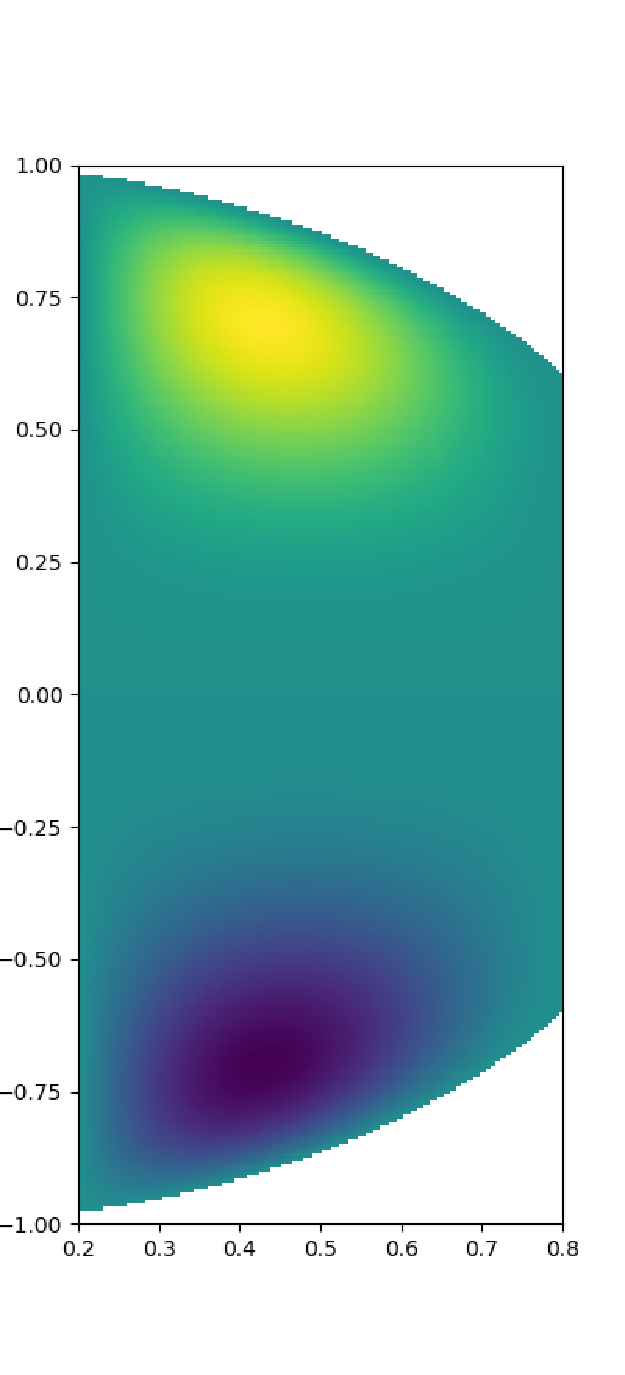
\includegraphics[scale=0.3]{solution-exact-poisson-diskslice-alpha=0p2-beta=0p8-u=y3expx-actual}
	\centering
	\end{subfigure}
	\begin{subfigure}{0.3\textwidth}
	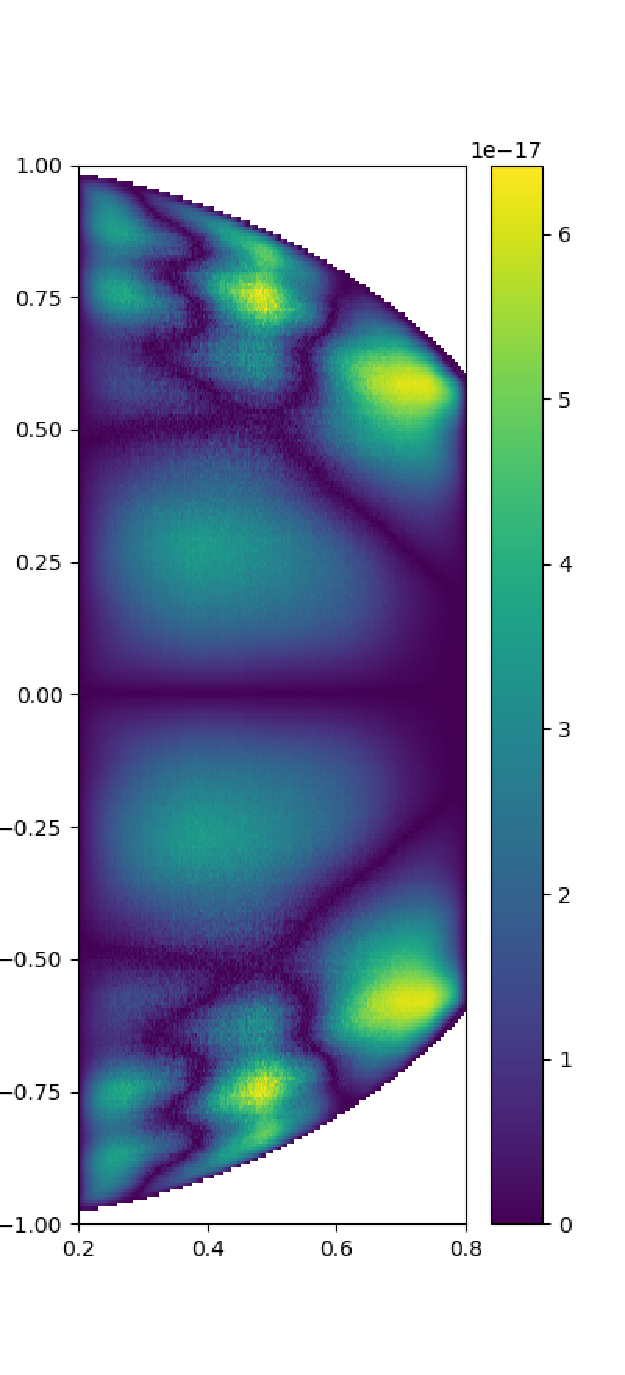
\includegraphics[scale=0.3]{solution-exact-poisson-diskslice-alpha=0p2-beta=0p8-u=y3expx-compare}
	\centering
	\end{subfigure}
	\centering
	\caption{The computed solution to $\Delta u = f$ with zero boundary conditions compared with the exact solution $u(x,y) = \Wiii (x,y) y^3 \exp(x)$. Left: Computed. Centre: Exact. Right: Plot of the error (colourbar is shown to demonstrate magnitude of the error is of the order $10^{-17}$)}
	\centering
	\label{fig:poissonexact}
\end{figure}

\begin{figure}[t]
	\begin{subfigure}{0.3\textwidth}
	\centering
	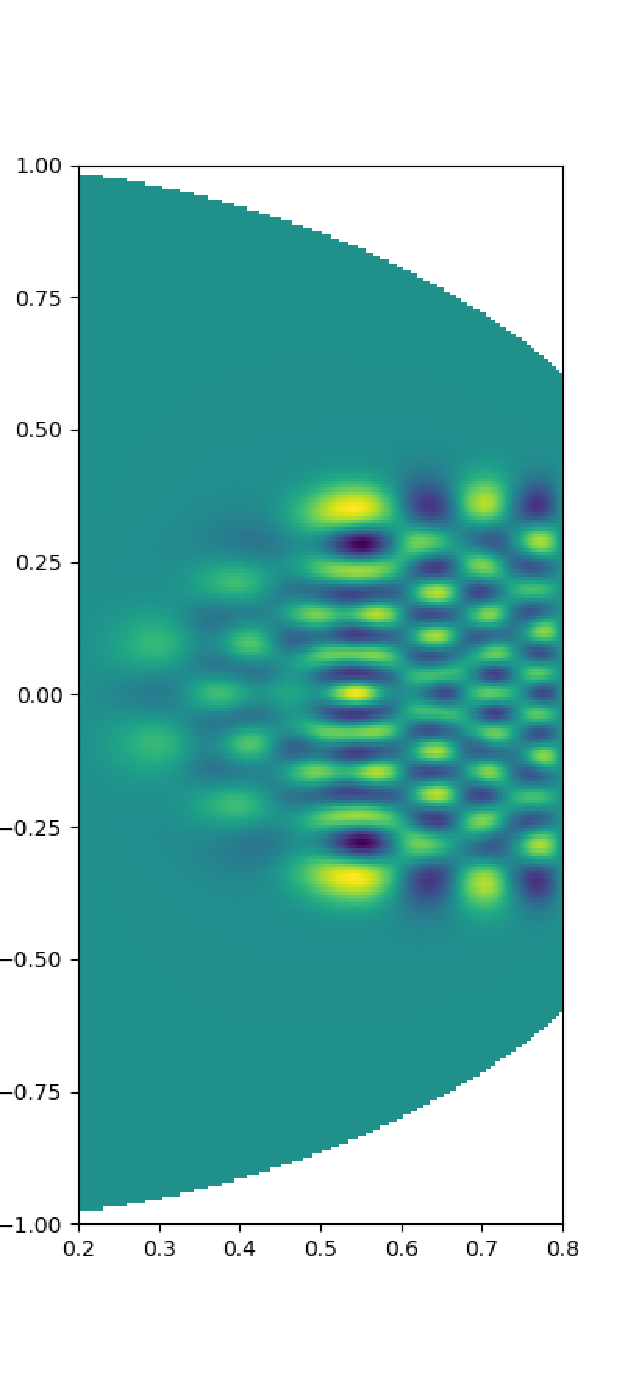
\includegraphics[scale=0.3]{solution-helmholtz-diskslice-alpha=0p2-beta=0p8-k=100-n=300}
	%\label{fig:solution-helmholtz}
	\end{subfigure}
	\begin{subfigure}{0.5\textwidth}
	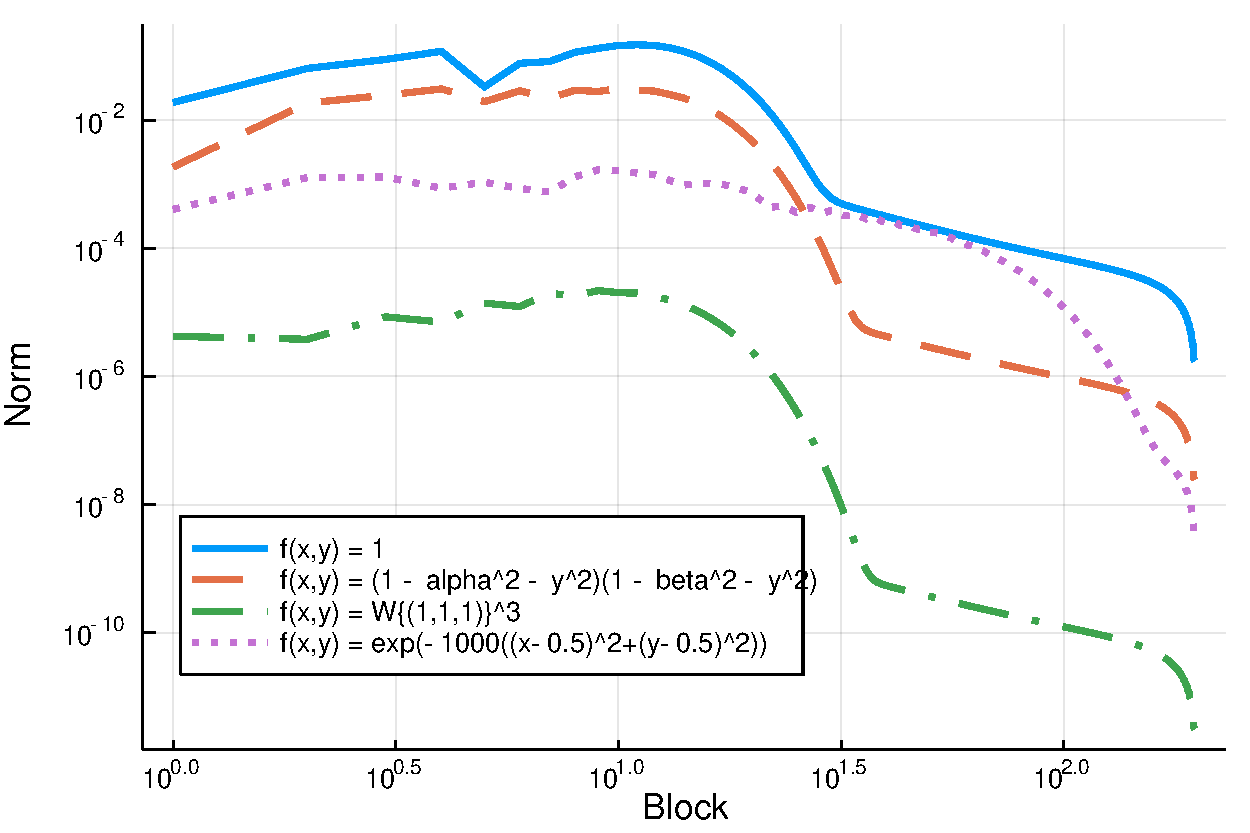
\includegraphics[scale=0.5]{solutionblocknorms-helmholtz-diskslice-alpha=0p2-beta=0p8-N=196-k=20}
	\centering
        	%\label{fig:solutionblocknorms-helmholtz}
	\end{subfigure}
	\caption{Left: The computed solution to $\Delta u + k^2 \: v \: u = f$ with zero boundary conditions with $f(x,y) = x(1-x^2-y^2)e^x$, $v(x,y) = 1 - (3(x-1)^2 + 5y^2)$ and $k = 100$. Right: The norms of each block of the computed solution of the Helmholtz equation with the given right hand side functions, with $k=20$ and $v(x,y) = 1 - (3(x-1)^2 + 5y^2)$.}
	\centering
	\label{fig:helmholtz}
\end{figure}

\begin{figure}[t]
	\begin{subfigure}{0.3\textwidth}
	\centering
	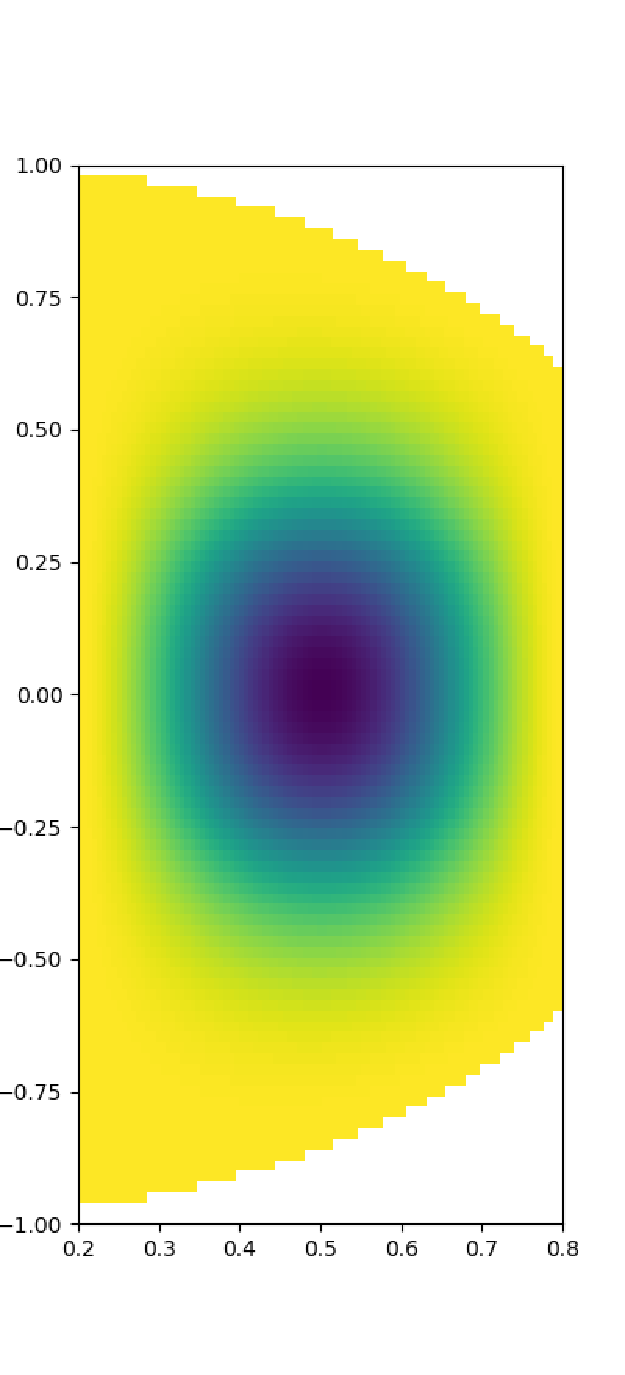
\includegraphics[scale=0.3]{solution-biharmonic-diskslice-alpha=0p2-beta=0p8}
	%\label{fig:solution-biharmonic}
	\end{subfigure}
	\begin{subfigure}{0.5\textwidth}
	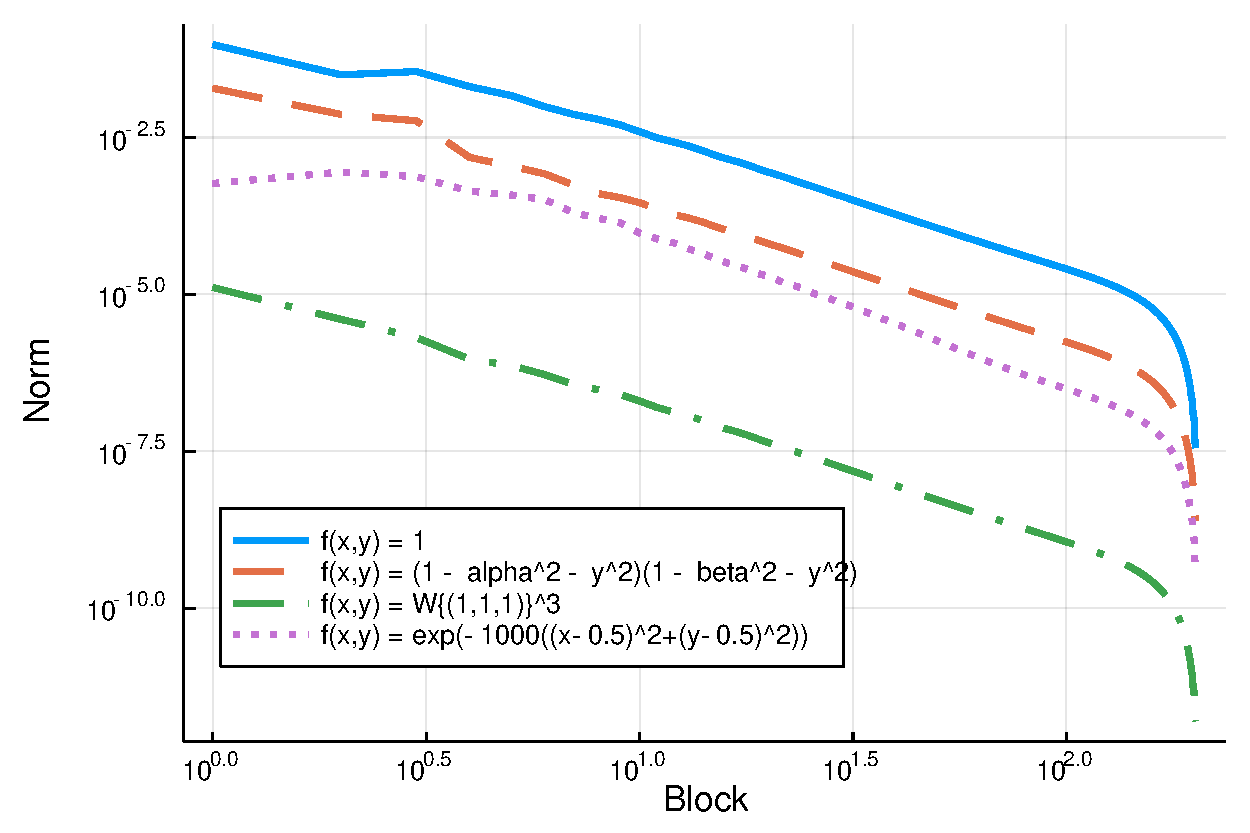
\includegraphics[scale=0.5]{solutionblocknorms-biharmonic-diskslice-alpha=0p2-beta=0p8-N=200}
	\centering
        	%\label{fig:solutionblocknorms-biharmonic}
	\end{subfigure}
	\caption{Left: The computed solution to $\Delta^2 u = f$ with zero Dirichlet and Neumann boundary conditions with $f(x,y) = 1 + \text{erf}(5(1 - 10((x - 0.5)^2 + y^2)))$. Right: The norms of each block of the computed solution of the biharmonic equation with the given right hand side functions.}
	\centering
	\label{fig:biharmonic}
\end{figure}
% END FIGURES

The Poisson equation is the classic problem of finding \(u(x,y)\) given a function \(f(x,y)\) such that:
\begin{align}
	\begin{cases}
    		\nabla^2 u(x,y,z) = f(x,y,z) &\quad \text{in } \Omega \\
		u(x,y,z) = 0& \quad \text{on } \partial \Omega
	\end{cases}.
	\label{eqn:poisson}
\end{align}
noting the imposition of zero Dirichlet boundary conditions on $u$.

We can tackle the problem as follows. Choose an $N \in \N$ large enough for the problem, and denote the coefficient vector for expansion of $u$ in the $\bigWNi$ OP basis up to degree $N$ by $\mathbf{u}$, and the coefficient vector for expansion of $f$ in the $\bigscopNi$ OP basis up to degree $N$ by $\mathbf{f}$. Since $f$ is known, we can obtain $\mathbf{f}$ using the quadrature rule in Section \ref{subsection:expandingfunctions}. In matrix-vector notation, our system hence becomes:
\begin{align*}
    \Delta_W^{(1)} \mathbf{u} = \mathbf{f}
\end{align*}
which can be solved to find $\mathbf{u}$.
In Figure \ref{fig:poisson} we see the solution to the Poisson equation with zero boundary conditions given in (\ref{eqn:poisson}) in the disk-slice $\Omega$. In Figure \ref{fig:poisson} we also show the norms of each block of calculated coefficients of the approximation for four right-hand sides of the Poisson equation with N = 200, that is, 20,301 unknowns. The rate of decay in the coefficients is a proxy for the rate of convergence of the computed solution: as typical of spectral methods, we expect the numerical scheme to converge at the same rate as the coefficients decay. We see that we achieve algebraic convergence for the first three examples, noting that for right hand-sides that vanish at the corners of our disk-slice ($x\in\{\alpha,\beta\}, \: y = \pm \rho(x)$) we observe faster convergence. \bstodo{get figs and update the comments here}

In Figure \ref{fig:poissonexact} we see an example where the solution calculated to the Poisson equation is shown together with a plot of the exact solution and the error. The example was chosen so that the exact solution was $u(x,y,z) = \genjacw^{(1,0)}(z) y^3 \exp(x)$, and thus the RHS function $f$ would be $f(x,y,z) = \Delta \big[\genjacw^{(1,0)}(z) y^3 \exp(x)\big]$. We see that the computed solution is almost exact. 


\subsection{Inhomogeneous variable-coefficient Helmholtz}

Find \(u(x,y)\) given functions $v$, $f : \Omega \to \R$ such that:
\begin{align}
	\begin{cases}
    		\nabla^2 u(x,y,z) + k^2 \: v(x,y,z) \; u(x,y,z) = f(x,y,z) &\quad \text{in } \Omega \\
		u(x,y,z) = 0 &\quad \text{on } \partial \Omega
	\end{cases}
	\label{eqn:helmholtz}
\end{align}
where $k \in \R$, noting the imposition of zero Dirichlet boundary conditions on $u$.

We can tackle the problem as follows. Denote the coefficient vector for expansion of $u$ in the $\bigWNi$ OP basis up to degree $N$ by $\mathbf{u}$, and the coefficient vector for expansion of $f$ in the $\bigscopNi$ OP basis up to degree $N$ by $\mathbf{f}$. Since $f$ is known, we can obtain  the coefficients $\mathbf{f}$ using the quadrature rule in Section \ref{subsection:expandingfunctions}. We can obtain the matrix operator for the variable-coefficient function $v(x,y,z)$ by using the Clenshaw algorithm with matrix inputs as the Jacobi matrices ${J_x^{(0)}}^\top, {J_y^{(0)}}^\top, {J_z^{(0)}}^\top$, yielding an operator matrix of the same dimension as the input Jacobi matrices a la the procedure introduced in \cite{olver2019triangle}. We can denote the resulting operator acting on coefficients in the $\bigscopNo$ space by $V({J_x^{(0)}}^\top, {J_y^{(0)}}^\top, {J_z^{(0)}}^\top)$. In matrix-vector notation, our system hence becomes:
\begin{align*}
    (\Delta_W^{(1)} + k^2 \:T^{(0)\to(1)} \: V \: T_W^{(1)\to(0)}) \: \mathbf{u} = \mathbf{f}
\end{align*}
which can be solved to find $\mathbf{u}$. We can see the sparsity and structure of this matrix system in Figure \ref{fig:sparsity} with $v(x,y,z) = zxy^2$ as an example. In Figure \ref{fig:helmholtz} we see the solution to the inhomogeneous variable-coefficient Helmholtz equation with zero boundary conditions given in (\ref{eqn:helmholtz}) in the half-disk $\Omega$, with $k=100$, $v(x,y,z) = 1 - (3(x-1)^2 + 5y^2)$ and $f(x,y,z) = x(1-x^2-y^2)e^x$. In Figure \ref{fig:helmholtz} we also show the norms of each block of calculated coefficients of the approximation for four right-hand sides of the inhomogeneous variable-coefficient Helmholtz equation with $k=20$ and $v(x,y,z) = 1 - (3(x-1)^2 + 5y^2)$ using N = 200, that is, 20,301 unknowns. The rate of decay in the coefficients is a proxy for the rate of convergence of the computed solution. We see that we achieve algebraic convergence for the first three examples, noting that for right hand sides that vanish at the corners of our disk-slice ($x\in\{\alpha,\beta\}, \: y = \pm \rho(x)$) we see faster convergence. \bstodo{get figs and update the comments here}

% For the final Gaussian bump example, we see that we achieve spectral convergence.

We can extend this to constant non-zero boundary conditions by simply noting that the problem 
\begin{align*}
	\begin{cases}
    		\nabla^2 u(x,y,z) + k^2 \: v(x,y,z) \; u(x,y,z) = f(x,y,z) &\quad \text{in } \Omega \\
		u(x,y,z) = c \in \R &\quad \text{on } \partial \Omega
	\end{cases}
\end{align*}
is equivalent to letting $u = \tilde{u} + c$ and solving
\begin{align*}
	\begin{cases}
    		\nabla^2 \tilde{u}(x,y,z) + k^2 \: v(x,y,z) \; \tilde{u}(x,y,z) = f(x,y,z) - c \: k^2 \: v(x,y,z) \; =: g(x,y,z)  \quad \text{in } \Omega \\
		\tilde{u}(x,y,z) = 0 \quad \text{on } \partial \Omega
	\end{cases}
\end{align*}
and solving this zero boundary condition Helmholtz problem.


\subsection{Biharmonic equation}

Find $u(x,y,z)$ given a function $f(x,y,z)$ such that:
\begin{align}
	\begin{cases}
    		\rho(z)^2 \: \Delta^2 u(x,y,z) = \rho(z)^2 \: f(x,y,z) &\quad \text{in } \Omega \\
		u(x,y,z) = 0, \quad \frac{\partial u}{\partial n}(x,y,z) = 0 &\quad \text{on } \partial \Omega
	\end{cases}
	\label{eqn:biharmonic}
\end{align}
where $\Delta^2$ is the Biharmonic operator, noting the imposition of zero Dirichlet and Neumann boundary conditions on $u$. In Figure \ref{fig:biharmonic} we see the solution to the Biharmonic equation (\ref{eqn:biharmonic}) in the disk-slice $\Omega$. In Figure \ref{fig:biharmonic} we also show the norms of each block of calculated coefficients of the approximation for four right-hand sides of the biharmonic equation with N = 200, that is, 20,301 unknowns.  We see that we achieve algebraic convergence for the first three examples, noting that for right hand sides that vanish at the corners of our disk-slice ($x\in\{\alpha,\beta\}, \: y = \pm \rho(x)$) we see faster convergence. \bstodo{get figs and update the comments here}

% For the final Gaussian bump example, we see that we achieve spectral convergence.


%
\section{Tangent space (vector-valued functions)}\label{Section:tangentspace}

We can extend the methodology detailed here to the tangent space of the spherical cap $\Omega$. By creating a basis of orthogonal vector-valued functions (OVFs) for the spherical cap $\Omega$, we can expand vector-valued functions that lie in tangent space we call $\tangentspace$ in this basis. Such functions that are useful for the sphere are gradients and perpendicular-gradients of scalar functions. In this section we will define the OVFs, outline the Clenshaw matrices and how to build the OVFs, function evaluation as well as differential operators for gradient, curl and divergence that take us to and from coefficients in either of the OVF or scalar OP expansions.

Any function in the tangent space of $\Omega$ can be written as $\nabla f + \rvec \times \nabla g$ for some scalar functions $f, g$ on $\Omega$. Let $f$ be a scalar function on $\Omega$ that satisfies zero boundary conditions. Then there exist coefficients $\bm{f}$ such that $f$ can be expanded in the OP basis $\bigW_N^{(1)}$ for large enough N, i.e. $f = \genjacw^{(1,0)} \: \sum_{n,k,i} f_{n,k,i} \: \scopnki^{(1)}$. The gradient and perpendicular gradient of $f$ are then
\begin{align*}
	\nabla f &= \sum_{n,k,i} f_{n,k,i} \: \nabla \Big( \genjacw^{(1,0)} \: \scopnki^{(1)} \Big) \\
	\rvec \times \nabla f &= \sum_{n,k,i} f_{n,k,i} \: \rvec \times \nabla \Big( \genjacw^{(1,0)} \: \scopnki^{(1)} \Big).
\end{align*}
The game is to find an orthogonal basis such that we can sparsely expand $\nabla \Big( \genjacw^{(1,0)} \: \scopnki^{(1)} \Big)$ and $\rvec \times \nabla \Big( \genjacw^{(1,0)} \: \scopnki^{(1)} \Big)$ for each $n,k,i$ trio.

Define the OVFs as follows:
\begin{align}
	\tsopinki(x,y,z) &:= \phivec \: \frac{1}{\rho(z)} \: \scopnki^{(0)}(x,y,z) \\
	\tsopiinki(x,y,z) &:= \thetavec \: \frac{1}{\rho(z)} \: \scopnki^{(0)}(x,y,z)
\end{align}
where
\begin{align}
	\phivec &:= 
		\begin{pmatrix}
			\cos(\theta) \: \cos(\phi) \\
			\sin(\theta) \: \cos(\phi) \\
			- \sin(\phi)
		\end{pmatrix}
		=
		\begin{pmatrix}
			x z / \rho(z) \\
			y z / \rho(z) \\
			- \rho(z)
		\end{pmatrix} \\
	\thetavec &:= 
		\begin{pmatrix}
			-\sin(\theta) \\
			\cos(\theta) \\
			0
		\end{pmatrix}
		=
		\begin{pmatrix}
			-y / \rho(z) \\
			x / \rho(z) \\
			0
		\end{pmatrix}
\end{align}
These are orthogonal with respect to the inner product $\ip<\bm{A}, \bm{B}>_\tangentspace := \int_\Omega \bm{A} \cdot \bm{B} \: \rho(z)^2 \:\D \Omega$:
\begin{align*}
	\ip<\tsopinki, \tsopi_{m,j,h}>_\tangentspace &= \int_\Omega \tsopinki \cdot \tsopi_{m,j,h} \: \rho(z)^2 \:\D \Omega \\
	&= \int_\Omega \scopnki^{(0)} \: \scopmjh^{(0)} \: \D \Omega \\
	&= \pi \: \normgenjac^{(0, 2k)} \: \delta_{n,m} \: \delta_{k,j} \: \delta_{i,h}, \\
	\ip<\tsopiinki, \tsopii_{m,j,h}>_\tangentspace &= \int_\Omega \tsopiinki \cdot \tsopii_{m,j,h} \: \rho(z)^2 \:\D \Omega \\
	&= \int_\Omega \scopnki^{(0)} \: \scopmjh^{(0)} \: \D \Omega \\
	&= \pi \: \normgenjac^{(0, 2k)} \: \delta_{n,m} \: \delta_{k,j} \: \delta_{i,h}, \\
	\ip<\tsopinki, \tsopii_{m,j,h}>_\tangentspace &\equiv 0.
\end{align*}
To show that these span the tangent space $\tangentspace$, we merely require that we can sparsely expand $\nabla \Big( \genjacw^{(1,0)} \: \scopnki^{(1)} \Big), \: \rvec \times \nabla \Big( \genjacw^{(1,0)} \: \scopnki^{(1)} \Big)$ with the vectors $\tsopi_{m,j,h}, \tsopii_{m,j,h}$.  First, note that
\begin{align*}
	\nabla \Big( \genjacw^{(1,0)} \: \scopnki^{(1)} \Big) &= \phivec \: \ppphi \Big( \genjacw^{(1,0)} \: \scopnki^{(1)} \Big) + \thetavec \: \frac{1}{\rho(z)} \: \pptheta \Big( \genjacw^{(1,0)} \: \scopnki^{(1)} \Big) \\
	&= \phivec \: \Big[k \: z \: \genjacw^{(1,0)}(z) \: \genjacnmk^{(1,2k)}(z) -  \big(\genjacw^{(1,0)}(z) \: \genjacnmk^{(1,2k)}(z) \big)' \rho(z)^2 \Big] \: \rho(z)^{k-1} \: \chki(\theta) \\
	&\quad \quad + \thetavec \: (-1)^{i+1} \: k \: \genjacw^{(1,0)}(z) \: \genjacnmk^{(1,2k)}(z) \: \rho(z)^{k-1} \: \ch_{k,|i-1|}(\theta).
\end{align*}
Then,
\begin{align*}
	&\ip<\nabla \Big( \genjacw^{(1,0)} \: \scopnki^{(1)} \Big), \tsopi_{m,j,h}>_\tangentspace \\
	&\quad \quad = \int_\Omega \nabla \Big( \genjacw^{(1,0)} \: \scopnki^{(1)} \Big) \cdot \tsopi_{m,j,h} \: \rho(z)^2 \:\D \Omega \\
	&\quad \quad = \pi \: \delta_{k,j} \: \delta_{i,h} \: \int_\alpha^1 \Big[k \: z \: \genjacw^{(1,0)} \: \genjacnmk^{(1,2k)} -  (\genjacw^{(1,0)} \: \genjacnmk^{(1,2k)})' \rho^2 \Big] \: \rho^{k-1} \: \genjac_{m-k}^{(0,2k)} \: \rho^{k-1} \: \rho^2 \:\D z \\
	&\quad \quad = \pi \: \delta_{k,j} \: \delta_{i,h} \: \int_\alpha^1 \Big[k \: z \: \genjacw^{(1,0)} \: \genjacnmk^{(1,2k)} -  (\genjacw^{(1,0)} \: \genjacnmk^{(1,2k)})' \rho^2 \Big] \: \genjac_{m-k}^{(0,2k)} \: \rho^{2k} \:\D z \quad (\star) \\
	&\quad \quad = \pi \: \delta_{k,j} \: \delta_{i,h} \: \int_\alpha^1 \Big( kz \: \genjacnmk^{(1,2k)} \: \genjac_{m-k}^{(0,2k)} \: \genjacw^{(1,2k)} \\
	&\quad \quad\quad \quad\quad \quad\quad \quad\quad \quad+ \genjacw^{(1,2k)} \: \genjacnmk^{(1,2k)} \: \Big[ \genjac_{m-k}^{(0,2k) \; \prime} \: \rho^2 - (2k+2) \: z \: \genjac_{m-k}^{(0,2k)} \Big] \Big) \: \D z \\
	&\quad \quad = \pi \: \delta_{k,j} \: \delta_{i,h} \: \int_\alpha^1 \genjacnmk^{(1,2k)} \: \Big[ - (k + 2) \: z \: \genjac_{m-k}^{(0,2k)} + \genjac_{m-k}^{(0,2k) \; \prime} \: \rho^2 \Big] \: \genjacw^{(1,2k)} \: \D z \quad (\star \star)
\end{align*}
where by orthogonality of the $\{\genjac_n^{(a,2b)}\}$ OPs we have that the above is zero for $m - k > n - k + 2 \iff m > n + 2$ at $(\star)$ and also for $n - k > m - k + 1 \iff m < n - 1$ at $(\star \star)$. Further, 
\begin{align*}
	&\ip<\nabla \Big( \genjacw^{(1,0)} \: \scopnki^{(1)} \Big), \tsopii_{m,j,h}>_\tangentspace \\
	&\quad \quad = \int_\Omega \nabla \Big( \genjacw^{(1,0)} \: \scopnki^{(1)} \Big) \cdot \tsopii_{m,j,h} \: \rho(z)^2 \:\D \Omega \\
	&\quad \quad = (-1)^{i+1} \: k \: \pi \: \delta_{k,j} \: \delta_{i,|h-1|} \: \int_\alpha^1 \genjacw^{(1,0)} \: \genjacnmk^{(1,2k)} \: \rho^{k-1} \: \genjac_{m-k}^{(0,2k)} \: \rho^{k-1} \: \rho^2 \:\D z \\
	&\quad \quad = (-1)^{i+1} \: k \: \pi \: \delta_{k,j} \: \delta_{i,|h-1|} \: \int_\alpha^1 \genjacnmk^{(1,2k)}  \: \genjac_{m-k}^{(0,2k)} \: \genjacw^{(1,2k)} \: \D z
\end{align*}
which again by orthogonality is zero for $m - k > n - k + 1 \iff m > n + 1$ and $n - k > m - k \iff m < n$. We of course have similar results for $\rvec \times \nabla \Big( \genjacw^{(1,0)} \: \scopnki^{(1)} \Big)$ since
\begin{align*}
	\rvec \times \phivec = \thetavec, \quad \rvec \times \thetavec = - \phivec.
\end{align*}
We now have a set of orthogonal vector valued functions that span the tangent space $\tangentspace$. By construction, we have the same recurrence coefficients for multiplication by $x,y,z$ for each of the OVFs as for the OPs $\scopnki^{(0)}$. 

Define
\begin{align*}
	\bigtsoptn := 
		\begin{pmatrix}
			\tsopit_{n,0,0}(x,y,z) \\
			\tsopiit_{n,0,0}(x,y,z) \\
			\tsopit_{n,1,0}(x,y,z) \\
			\tsopiit_{n,1,0}(x,y,z) \\
			\tsopit_{n,1,1}(x,y,z) \\
			\tsopiit_{n,1,1}(x,y,z) \\
			\vdots \\
			\tsopit_{n,n,0}(x,y,z) \\
			\tsopiit_{n,n,0}(x,y,z) \\
			\tsopit_{n,n,1}(x,y,z) \\
			\tsopiit_{n,n,1}(x,y,z)
		\end{pmatrix} \in \R^{2(2n+1) \times 3}, 
	\quad \quad 
	\bigtsopt := 
		\begin{pmatrix}
			\bigtsopt_0 \\
			\bigtsopt_1 \\
			\bigtsopt_2 \\
			\vdots \\
		\end{pmatrix}
\end{align*}
and set $\jacobimattangentx, \jacobimattangenty, \jacobimattangentz$ as the Jacobi matrices corresponding to
\begin{align}
	\jacobimattangentx \: \bigtsopt(x,y,z) = x \: \bigtsopt(x,y,z), \nonumber \\
	\jacobimattangenty \: \bigtsopt(x,y,z) = y \: \bigtsopt(x,y,z), \label{eqn:jacobimatricestangentdefinition} \\
	\jacobimattangentz \: \bigtsopt(x,y,z) = z \: \bigtsopt(x,y,z), \nonumber
\end{align}
The matrices $\jacobimattangentx, \jacobimattangenty, \jacobimattangentz$ act on the coefficients vector of a function's expansion in the $\bigtsopt$ basis. For example, let a function $\bm{F}(x,y,z) : \Omega \to \tangentspace$ be approximated by its expansion $\bm{F}(x,y,z)^\top = \bigtsopt(x,y,z)^\top \bm{F}_c$, for some coefficients vector $\bm{F}_c$. Then $x \: \bm{F}(x,y,z)$ is approximated by $\bigtsopt(x,y,z)^\top {(\jacobimattangentx)}^\top \bm{F}_c$. In other words, ${(\jacobimattangentx)}^\top \bm{F}_c$ is the coefficients vector for the expansion of the function $(x,y,z) \mapsto x \: \bm{F}(x,y,z)$ in the  $\bigtsopt$ basis. Further, note that $\jacobimattangentx, \jacobimattangenty, \jacobimattangentz$ are banded-block-banded matrices -- they are block-tridiagonal (block-bandwidths $(1,1)$):
\begin{align*}
	\jacobimattangent_{x/y/z} &= 
		\begin{pmatrix}
			B_{x/y/z, 0} & A_{x/y/z, 0} & & & & \\
			C_{x/y/z, 1} & B_{x/y/z, 1} & A_{x/y/z, 1} & & & \\
			& C_{x/y/z, 2} & B_{x/y/z, 2} & A_{x/y/z, 2} & & & \\
			& & C_{x/y/z, 3} & \ddots & \ddots & \\
			& & & \ddots & \ddots & \ddots \\
		\end{pmatrix}
\end{align*}
For $\jacobimattangentx$, the sub-blocks have sub-block-bandwidths $(?,?)$:
\begin{align*}
	A_{x,n} &:= 
		\begin{pmatrix}
			0 & A_{n,0,6} & 0 & & \\
			A_{n,1,5} & \ddots & \ddots & & \\
			& \ddots & \ddots & \ddots & \\
			& & A_{n,n,5} & 0 & A_{n,n,6} \\
		\end{pmatrix} \in \R^{2(2n+1)\times2(2n+3)}, \quad n = 0,1,2,\dots \\
	B_{x,n} &:= 
		\begin{pmatrix}
			0 & A_{n,0,4} & & \\
			A_{n,1,3} & \ddots & \ddots & \\
			& \ddots & \ddots & A_{n,n-1,4} \\
			& & A_{n,n,3} & 0
		\end{pmatrix} \in \R^{2(2n+1)\times2(2n+1)}  \quad n = 0,1,2,\dots \\
	C_{x,n} &:= 
		\begin{pmatrix}
			0 & A_{n,0,2} & & \\
			A_{n,1,1} & \ddots & \ddots & \\
			& \ddots & \ddots & A_{n,n-2,2} \\
			& & \ddots & 0 \\
			& & & A_{n,n,1} \\
		\end{pmatrix} \in \R^{2(2n+1)\times2(2n-1)}, \quad n = 1,2,\dots
\end{align*}
where
\begin{align*}
	A_{n,k,j} &:= \alphaonkj \: I_{4} \in \R^{4\times4}, \quad k = 1,\dots,n \: (j \text{ even}), \quad k = 2,\dots,n \: (j \text{ odd}) \\
	A_{n,0,j} &:=
		\begin{pmatrix}
			\alphao_{n,0,j} & 0 & 0 & 0 \\
			0 & \alphao_{n,0,j} & 0 & 0
		\end{pmatrix} \in \R^{2\times4}, \quad j \text{ even} \\
	A_{n,1,j} &:=
		\begin{pmatrix}
			\alphao_{n,1,j} & 0 \\
			0 & \alphao_{n,1,j} \\
			0 & 0 \\
			0 & 0
		\end{pmatrix} \in \R^{4\times2}, \quad j \text{ odd}
\end{align*}
For $\jacobimattangenty$, the sub-blocks have sub-block-bandwidths $(?,?)$:
\begin{align*}
	A_{y,n} &:= 
		\begin{pmatrix}
			0 & B_{n,0,6} & 0 & & \\
			B_{n,1,5} & \ddots & \ddots & & \\
			& \ddots & \ddots & \ddots & \\
			& & B_{n,n,5} & 0 & B_{n,n,6} \\
		\end{pmatrix} \in \R^{2(2n+1)\times2(2n+3)}, \quad n = 0,1,2,\dots \\
	B_{y,n} &:= 
		\begin{pmatrix}
			0 & B_{n,0,4} & & \\
			B_{n,1,3} & \ddots & \ddots & \\
			& \ddots & \ddots & B_{n,n-1,4} \\
			& & B_{n,n,3} & 0
		\end{pmatrix} \in \R^{2(2n+1)\times2(2n+1)}  \quad n = 0,1,2,\dots \\
	C_{y,n} &:= 
		\begin{pmatrix}
			0 & B_{n,0,2} & & \\
			B_{n,1,1} & \ddots & \ddots & \\
			& \ddots & \ddots & B_{n,n-2,2} \\
			& & \ddots & 0 \\
			& & & B_{n,n,1} \\
		\end{pmatrix} \in \R^{2(2n+1)\times2(2n-1)}, \quad n = 1,2,\dots
\end{align*}
where
\begin{align*}
	B_{n,k,j} &:= 
		\begin{pmatrix}
			0 & 0 & \betaonkj & 0 \\
			0 & 0 & 0 & \betaonkj \\
			\betaonkj & 0 & 0 & 0 \\
			0 & \betaonkj & 0 & 0
		\end{pmatrix} \in \R^{4\times4}, \quad k = 1,\dots,n \: (j \text{ even}), \quad k = 2,\dots,n \: (j \text{ odd}) \\
	B_{n,0,j} &:=
		\begin{pmatrix}
			0 & 0 & \betao_{n,0,j} & 0 \\
			0 & 0 & 0 & \betao_{n,0,j}
		\end{pmatrix} \in \R^{2\times4}, \quad j \text{ even} \\
	B_{n,1,j} &:=
		\begin{pmatrix}
			0 & 0 \\
			0 & 0 \\
			\betao_{n,1,j} & 0 \\
			0 & \betao_{n,1,j}
		\end{pmatrix} \in \R^{4\times2}, \quad j \text{ odd}
\end{align*}
For $\jacobimattangentz$, the sub-blocks have sub-block-bandwidths $(?,?)$:
\begin{align*}
	A_{z,n} &:= 
		\begin{pmatrix}
			\Gamma_{n,0,3} & 0 & 0 & & \\
			0 & \ddots & \ddots & & \\
			& \ddots & \ddots & \ddots & \\
			& & 0 & \Gamma_{n,n,3} & 0 \\
		\end{pmatrix} \in \R^{2(2n+1)\times2(2n+3)}, \quad n = 0,1,2,\dots \\
	B_{z,n} &:= 
		\begin{pmatrix}
			\Gamma_{n,0,2} & 0 & & \\
			0 & \ddots & \ddots & \\
			& \ddots & \ddots & 0 \\
			& & 0 & \Gamma_{n,n,2}
		\end{pmatrix} \in \R^{2(2n+1)\times2(2n+1)}  \quad n = 0,1,2,\dots \\
	C_{z,n} &:= 
		\begin{pmatrix}
			\Gamma_{n,0,1} & 0 & & \\
			0 & \ddots & \ddots & \\
			& \ddots & \ddots & 0 \\
			& & \ddots &  \Gamma_{n,n-1,1} \\
			& & & 0 \\
		\end{pmatrix} \in \R^{2(2n+1)\times2(2n-1)}, \quad n = 1,2,\dots
\end{align*}
where
\begin{align*}
	\Gamma_{n,k,j} &:= \gammaonkj \: I_{4} \in \R^{4\times4}, \quad k = 1,\dots,n \\
	\Gamma_{n,0,j} &:=
		\begin{pmatrix}
			\gammao_{n,0,j} & 0 \\
			0 & \gammao_{n,0,j}
		\end{pmatrix} \in \R^{2\times2}.
\end{align*}
Note that the sparsity of the Jacobi matrices (in particular the sparsity of the sub-blocks) comes from the natural sparsity of the three-term recurrences of the 1D OPs and the circular harmonics, meaning that the sparsity is not limited to the specific spherical cap, and would extend to the spherical band.


\subsection{Building the OPs} 

We can combine each system in (\ref{eqn:jacobimatricestangentdefinition}) into a block-tridiagonal system, for any $(x,y,z) \in \Omega$:

\begin{align*}
\renewcommand\arraystretch{1.3}
\begin{pmatrix}
		I_2 & & & \\
		B_0-G_0(x,y,z) & A_0 & & \\
		C_1 & B_1-G_1(x,y,z) & \quad A_1 \quad & \\
		& C_2 & B_2 - G_2(x,y,z)  & \ddots \\
		& & \ddots &\ddots
\end{pmatrix}
\bigtsopt(x,y,z)
=
\begin{pmatrix}
	 \tsopi_0^\top \\ \tsopii_0^\top \\ 0 \\ 0 \\ \vdots  \\
\end{pmatrix},
\end{align*}
where we note $\scopa_{0,0,0}(x,y,z) =: \scopa_0 \equiv \genjac_0^{(a,0)} \: \ch_0$, and for each $n = 0,1,2\dots$,
\begin{align*}
A_n &:= \begin{pmatrix}
		A_{x,n} \\
		A_{y,n} \\
		A_{z,n}
	    \end{pmatrix} \in \R^{6(2n+1)\times2(2n+3)}, \quad
C_n := \begin{pmatrix}
		C_{x,n} \\
		C_{y,n} \\
		C_{z,n}
	    \end{pmatrix} \in \R^{6(2n+1)\times2(2n-1)} \quad (n \ne 0), \nonumber \\
B_n &:= \begin{pmatrix}
		B_{x,n} \\
		B_{y,n} \\
		B_{z,n}
	    \end{pmatrix} \in \R^{6(2n+1)\times2(2n+1)}, \quad
G_n(x,y,z) := \begin{pmatrix}
		xI_{2(2n+1)} \\
		yI_{2(2n+1)} \\
		zI_{2(2n+1)}
	    \end{pmatrix} \in \R^{6(2n+1)\times2(n+1)}.
\end{align*}
 
For each $n = 0,1,2\dots$ let $\Dnt$ be any matrix that is a left inverse of $A_n$, i.e. such that $\Dnt A_n = I_{2(2n+3)}$. Multiplying our system by the preconditioner matrix that is given by the block diagonal matrix of the $\Dnt$'s, we obtain a lower triangular system \cite[p78]{dunkl2014orthogonal}, which can be expanded to obtain the recurrence:
\begin{align*}
	\begin{cases}
		\bigtsopt_{-1}(x,y,z) := 0 \\
		\bigtsopt_{0}(x,y,z) = 
			\begin{pmatrix} 
				\tsopi_0^\top \\ 
				\tsopii_0^\top
			\end{pmatrix} :=
			\begin{pmatrix} 
				\tsopi_{0,0,0}^\top \\
				\tsopi_{0,0,0}^\top
			\end{pmatrix} \\
		\bigtsopt_{n+1}(x,y,z) = -\Dnt (B_n-G_n(x,y,z)) \bigtsoptn(x,y,z) - \Dnt C_n  \, \bigtsopt_{n-1}(x,y,z), \quad n = 0,1,2,\dots.
	\end{cases}
\end{align*}

Note that we can define an explicit \(\Dnt\) as follows: \bstodo{type up DnT for tangent space}
\begin{align*}
\Dnt := \begin{pmatrix}
		0 & & & 0 & & & 1 / \gammaa_{n,0,3} & & \\
		& \ddots & & & \ddots & & & \ddots \\
		& & 0 & & & 0 & & & 1 / \gammaa_{n,n,3}  \\
		& & & & & \underline{\eta}^\top_{1} & & & \\
		& & & & & \underline{\eta}^\top_{0} & & &
	    \end{pmatrix} \in \R^{(2n+3)\times3(2n+1)},
\end{align*}
for $n = 2, 3, \dots$ where $\underline{\eta}_{0}, \underline{\eta}_{1} \in \R^{3(2n+1)}$ with entries given by 
\begin{align*}
	\big(\underline{\eta}_{0}\big)_j &= 
		\begin{cases}
			\frac{1}{\alphaa_{n,n,6}} & j = 2n+1 \\
			\frac{- \: \alphaa_{n,n,5}}{\alphaa_{n,n,6} \: \gammaa_{n, n-1, 3}} & j = 3(2n+1) - 2 \\
			0 & o/w
		\end{cases} \\
	\big(\underline{\eta}_{1}\big)_j &= 
		\begin{cases}
			\big(\underline{\eta}_{0}\big)_{j+1} & j = 2n, 3(2n+1) - 3 \\
			0 & o/w
		\end{cases}
\end{align*}
For $n=0, 1$, we can simply take
\begin{align*}
D^\top_0 &:= \begin{pmatrix}
		0 & 0 & \frac{1}{\gammaa_{0,0,3}} \\
		\frac{1}{\alphaa_{0,0,6}} & 0 & 0 \\
		0 & \frac{1}{\betaa_{0,0,6}} & 0
	    \end{pmatrix} \in \R^{3\times3}, \\
D^\top_1 &:= \begin{pmatrix}
		0 & 0 & 0 & 0 & 0 & 0 & 1 / \gammaa_{1,0,3} & & \\
		0 & 0 & 0 & 0 & 0 & 0 & 0 & 1 / \gammaa_{1,1,3} \\
		0 & 0 & 0 & 0 & 0 & 0 & 0 & 0 & 1 / \gammaa_{1,1,3}  \\
		0 & 1 / \alphaa_{1,1,6} & 0 & 0 & 0 & 0 & \eta & 0 & 0 \\
		0 & 0 & 1 / \alphaa_{1,1,6} & 0 & 0 & 0 & 0 & 0 & 0
	    \end{pmatrix} \in \R^{5\times9},
\end{align*}
where $\eta = \frac{- \: \alphaa_{1,1,5}}{\alphaa_{1,1,6} \: \gammaa_{1, 0, 3}}$.

It follows that we can apply $\Dnt$ in $O(n)$ complexity, and thereby calculate $\bigtsopt_0(x,y,z)$  through $\bigtsoptn(x,y,z)$ in optimal $O(n^2)$ complexity. \bstodo{correct for this case}

\subsection{Operators}

Gradient operator on a scalar function is pretty much outlined above. Divergence would either be worked out by knowing what $f,g$ are for a function $\bm{F} = \nabla f + \rvec \times \nabla g$, so that $\nabla \cdot \bm{F} = \nabla^2 f$. Alternatively, we have expressions for $\rhoppphi \scopnkia$ and $\pptheta \scopnkia$ so that we can calculate an operator for $\rho^2 \nabla \cdot$, i.e. 
\begin{align*}
	\rho^2 \nabla \cdot \bm{F} &= \rho^2 \: \frac{1}{\rho} \ppphi (\rho F^\phi) + \rho^2 \: \frac{1}{\rho} \pptheta F^\theta \\
	&= \sum_{n,k,i} F^\phi_{n,k,i} \: \rhoppphi \scopnki^{(0)} + F^\theta_{n,k,i} \: \pptheta \scopnki^{(0)}.
\end{align*}

\bstodoinline{My main concern is whether this vector function basis is correct/valid. In my mind I would rather something like. I have found it difficult to come up with something that gives orthogonal vectors while still maintaining a sparse expansion for the gradient of a function. I am also confused about what the rho factors "mean".}





%
\section{Conclusions}

We have shown that tri-variate orthogonal polynomials can lead to sparse discretizations of general linear PDEs on spherical cap domains, with Dirichlet boundary conditions on the $z = \alpha \in (0,1)$ boundary. This work provides a detailed practical framework for the application of the methods described for quadratic surfaces of revolution \cite{olver2020orthogonal}, by utilising the non-classical 1D OPs on the interval $[\alpha, 1]$ with the weight $(z - \alpha)^a \: \sqrt{(1-z^2)}^b$ defined for the disk-slice case \cite{snowball2019sparse}. This work also forms a building block in developing an $hp-$finite element method to solve PDEs on the sphere by using spherical band and spherical cap shaped elements.

This work serves as a stepping stone to constructing similar methods to solve partial differential equations on other 3D sub-domains of the sphere - t is clear from the construction in this paper that discretizations of spherical gradients and Laplacian's are sparse on other suitable sub-components of the sphere. The resulting sparsity in high-polynomial degree discretizations presents an attractive alternative to methods based on bijective mappings (e.g., \cite{DGShallowWater,FEMShallowWater,boyd2005sphere}). Constructing these sparse spectral methods for surface PDEs on spherical bands and spherical triangles is future work, and has applications in weather prediction \cite{staniforth2012horizontal}.


%\noindent{\bf Acknowledgements}:  We would like to thank the anonymous referees for their helpful comments.  The second author was supported in part by the Leverhulme Trust Research Project Grant RPG-2019-144 ``Constructive approximation theory on and inside algebraic curves and surfaces.


%
\appendix
%
\section{P-finite element methods using sparse operators}\label{Appendix:PFEM}

\begin{figure}[t]
	\begin{subfigure}{0.3\textwidth}
	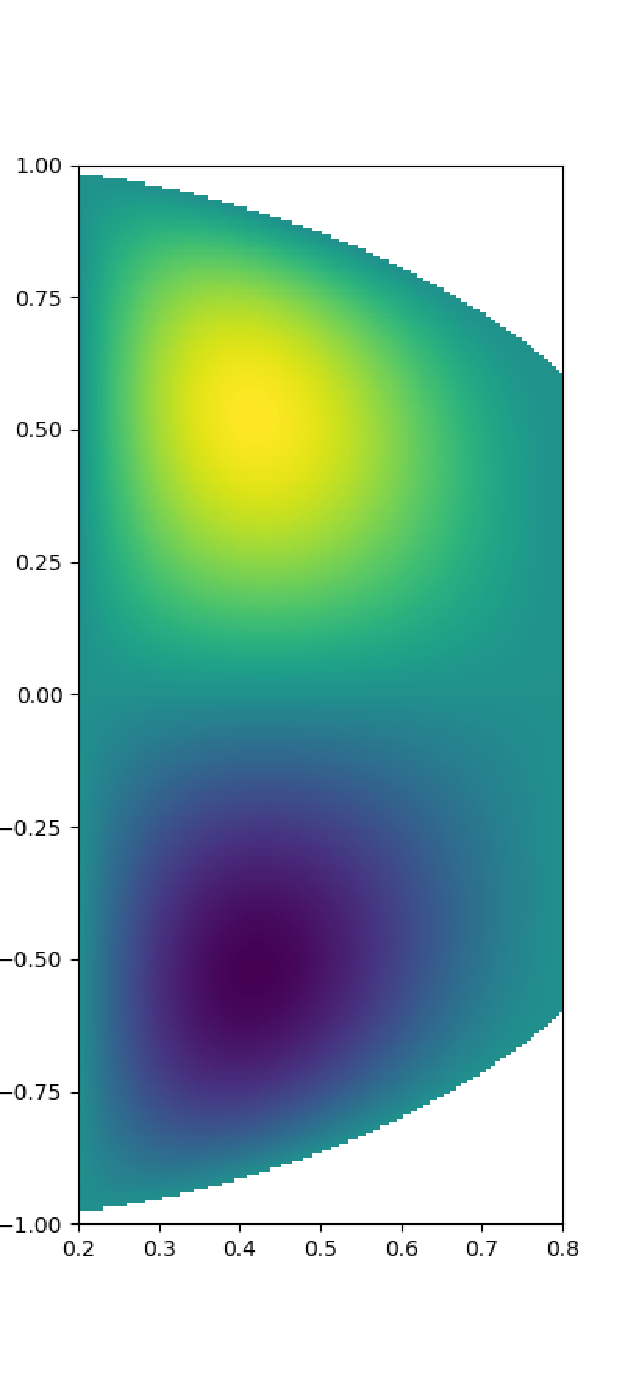
\includegraphics[scale=0.28]{solution-pfem-poisson-diskslice-alpha=0p2-beta=0p8-f=Wycosx}
        	%\label{fig:solutionblocknorms-poisson}
	\centering
	\end{subfigure}
	\begin{subfigure}{0.3\textwidth}
	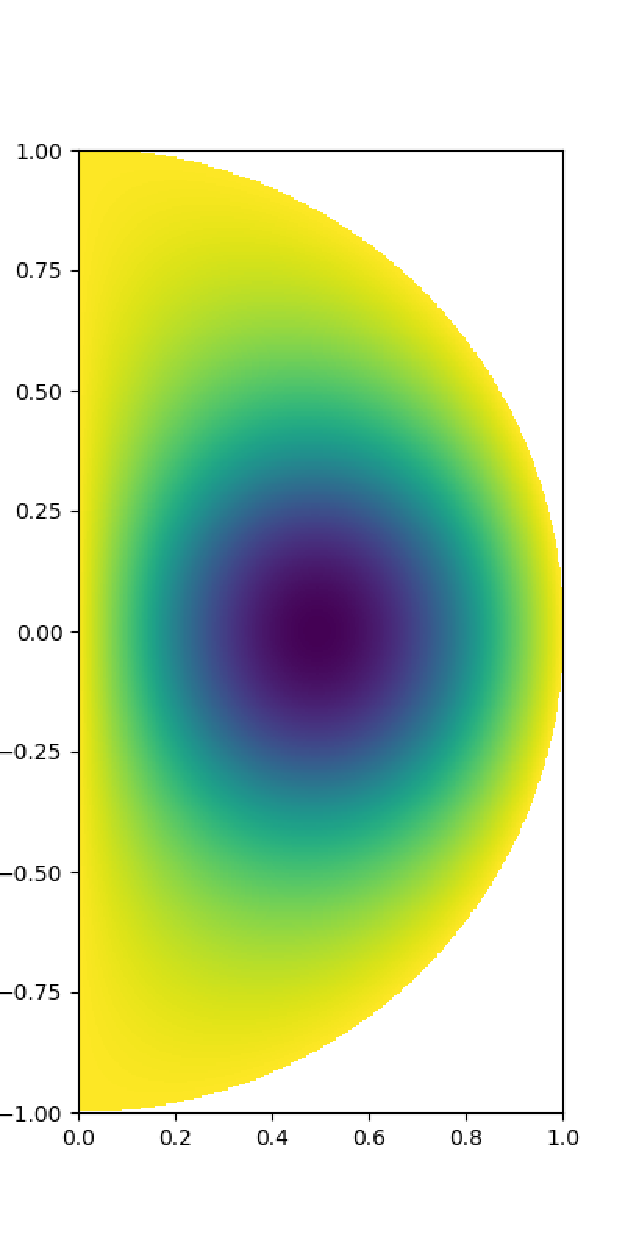
\includegraphics[scale=0.3]{solution-poisson}
	\centering
	%\label{fig:solution-poisson}
	\end{subfigure}
	\begin{subfigure}{0.3\textwidth}
	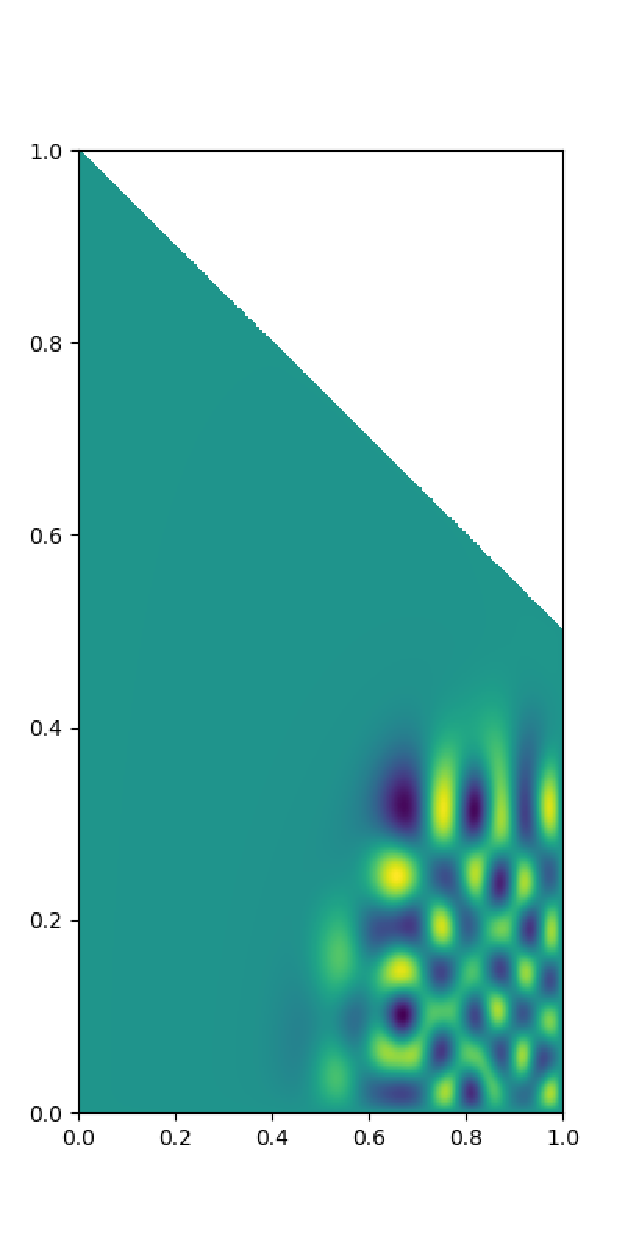
\includegraphics[scale=0.3]{solution-trapezium-helmholtz-k=100-n=1500}
	%\label{fig:solution-poisson}
	\centering
	\end{subfigure}
	\centering
	\caption{Left: The computed solution to $\Delta u = f$ with zero boundary conditions with $f(x,y) = \Wiii(x,y) y \cos(x)$ in the disk-slice using the $p$-FEM approach with a single element. Centre: The computed solution to $\Delta u = f$ with zero boundary conditions with $f(x,y) = 1 + \text{erf}(5(1 - 10((x - 0.5)^2 + y^2)))$ in the half-disk. Right: The computed solution to $\Delta u + k^2 \: v \: u = f$ with zero boundary conditions with $f(x,y) = (1-x) \: x \: y \: (1- \half x - y) \: e^x$, $v(x,y) = 1 - (3(x-1)^2 + 5y^2)$ and $k = 100$. in the trapezium.}
	\centering
	\label{fig:appendixfigs}
\end{figure}

We follow the method of \cite{beuchler2006new} to construct a sparse $p$-finite element method in terms of the operators constructed above, with the benefit of ensuring that the resulting discretisation is symmetric. Consider the 3D Dirichlet problem on a domain $\Omega$:
\begin{align*}
	\begin{cases}
         - \rho(z)^2 \: \nabla^2 u(x,y,z) = \rho(z)^2 \: f(x,y,z) \quad \text{in } \Omega \\
         u = 0 \quad \text{on } \partial \Omega
         \end{cases}
\end{align*}
This has the weak formulation
\begin{align*}
	L(v) := \int_\Omega \rho^2 \: f \: v \: \D \sigma(x,y) \D z = \int_\Omega \big(\rho \: \nabla u\big) \cdot \big(\rho \: \nabla v\big) \: \D \sigma(x,y) \D z =: a(u,v)
\end{align*}
 for any test function $v \in V := H_0^1(\Omega) = \{v \in H^1(\Omega) \quad | \quad v|_{\partial \Omega} = 0 \}$.

In general, we would split a sphere domain into spherical band elements with spherical caps over the poles, and use a $p$-finite element method to solve PDEs on the sphere using these elements $\{\element_n\}$. While spherical bands are an extension to this work, we note that we can still apply a $p$-FEM using two half-spheres ($\alpha = 0$). In this section, we limit our discretisation to a single element, that is we let $\element = \Omega$ for a spherical cap domain. We can choose our finite dimensional space $V_p = \{v_p \in V \quad | \quad {\rm deg}\,(v_p|_\element) \le p\}$ for some $p \in \N$.

We seek $u_p \in V_p$ s.t.
\begin{align}
	L(v_p) = a(u_p,v_p) \quad \forall \: v_p \in V_p.
	\label{eqn:FEMweakform}
\end{align}

Define $\Lambda^{(a)} :=  \ip< \bigscopa_p, \: {\bigscopa_p}^\top >_{\scopa}$ for any $a$. Note that due to orthogonality this is a diagonal matrix. By choosing suitable bases for our FE spaces, we can rewrite (\ref{eqn:FEMweakform}) in matrix-vector form. We can choose a basis for $V_p$ by using the weighted orthogonal polynomials on $\element$ with parameter $a = 1$, the $\bigW_p^{(1)}$ OPs, and we can expand the function $f$ in the $\bigscopi_p$ basis. 

Let $\mathbf{u}, \mathbf{v}$ be the coefficient vectors of the expansions of $u_p, v_p \in V_p$ respectively in the $V_p$ basis ($\bigWiii$ OPs). Then,
\begin{align*}
	a(u_p,v_p) &= \int_\element \big(\rho \: \nabla u\big) \cdot \big(\rho \: \nabla v\big) \: \D \sigma(x,y) \D z \\
	&= \int_\element \Big( \rhoppphi u_p \: \rhoppphi v_p + \pptheta u_p \: \pptheta v_p \Big) \: \D \sigma(x,y) \D z \\
	&= \int_\element \Big( \mathbf{v}^\top {W_\phi^{(1)}}^\top \bigscopo_p {\bigscopo_p}^\top W_\phi^{(1)} \mathbf{u} \nonumber \\
					& \quad \quad \quad + \mathbf{v}^\top ({T_W^{(1)\to(0)} D_\theta})^\top \bigscopa_p {\bigscopa_p}^\top T_W^{(1)\to(0)} D_\theta \mathbf{u}  \Big) \: \D \sigma(x,y) \D z \\
	&= \mathbf{v}^\top \: \Big( {W_\phi^{(1)}}^\top \Lambda^{(0)}  W_\phi^{(1)} + ({T_W^{(1)\to(0)} D_\theta})^\top \Lambda^{(0)} T_W^{(1)\to(0)} D_\theta \Big) \: \mathbf{u}.
\end{align*}
Further, let $\mathbf{f}$ is the coefficient vector for the expansion of the function $f(x,y,z)$ in the $\bigscopi_p$ OP basis and let $P$ be the operator for multiplication by $\rho(z)^2$, that is the operator matrix defined by $P^\top \bigscopi_p = \rho(z) \: \bigscopi_p$. Then,
\begin{align*}
	L(v_p) &= \int_\element \: v_p \: \rho^2 \: f \: \D \sigma(x,y) \D z \\
	&= \int_\element \: \mathbf{v}^\top \: \bigW_p^{(1)} \: {\bigscopi_p}^\top \: P \: \mathbf{f} \: \D \sigma(x,y) \D z \\	
	&= \mathbf{v}^\top \Lambda^{(1)} \: P \: \mathbf{f}.
\end{align*}

Since (\ref{eqn:FEMweakform}) is equivalent to stating that
\begin{align*}
	L(\genjacw^{(1)} \scopnkii) = a(u_p, \genjacw^{(1)} \scopnkii) \quad \forall \: n = 0,\dots,p, \: k = 0,\dots,n, \: i = 0,1
\end{align*}
(i.e. holds for all basis functions of $V_p$) by choosing $v_p$ as each basis function, we can equivalently write the linear system for our finite element problem as:
\begin{align*}
	A\mathbf{u} = \tilde{\mathbf{f}}.
\end{align*}
where the (element) stiffness matrix $A$ is defined by 
\begin{align*}
	A =  {W_\phi^{(1)}}^\top \Lambda^{(0)}  W_\phi^{(1)} + ({T_W^{(1)\to(0)} D_\theta})^\top \Lambda^{(0)} T_W^{(1)\to(0)} D_\theta
\end{align*}
and the load vector $\tilde{\mathbf{f}}$ is given by 
\begin{align*}
	\tilde{\mathbf{f}} = \Lambda^{(1)} \: P \: \mathbf{f}.
\end{align*}
Note that since we have sparse operator matrices for partial derivatives and basis-transform, we obtain a symmetric sparse (element) stiffness matrix, as well as a sparse operator matrix for calculating the load vector (rhs).



\bibliography{spherical-caps}


\end{document}











  







